\section{\Large PROBLEM SET 5}

\subsection{Problem 1 - Gravity Gradient Torque (Stability)}

\subsubsection{Calculate the coefficients Ki of the moments of inertia which drive stability under gravity gradient. Compute and plot regions of stable and unstable motion.}

Using Demos, an online graphing calculator tool, the plot shown in Figure \ref{fig:grav_gradient_stability} was produced. As shown in annotations on the figure, this plot represents regions in the $k_Tk_R$ plane for which stability is achieved. The equilibrium point about which this stability is described is one in which the principal axes of the spacecraft are aligned with the RTN frame, and the angular velocity of the spacecraft expressed in the principal frame is $\vec{\omega} = \begin{bmatrix} 0 & 0 & n \end{bmatrix}^T$, where $n$ is the mean motion of the spacecraft in its orbit. 

\begin{figure}[H]
    \centering
    \captionsetup{ justification = centering}
    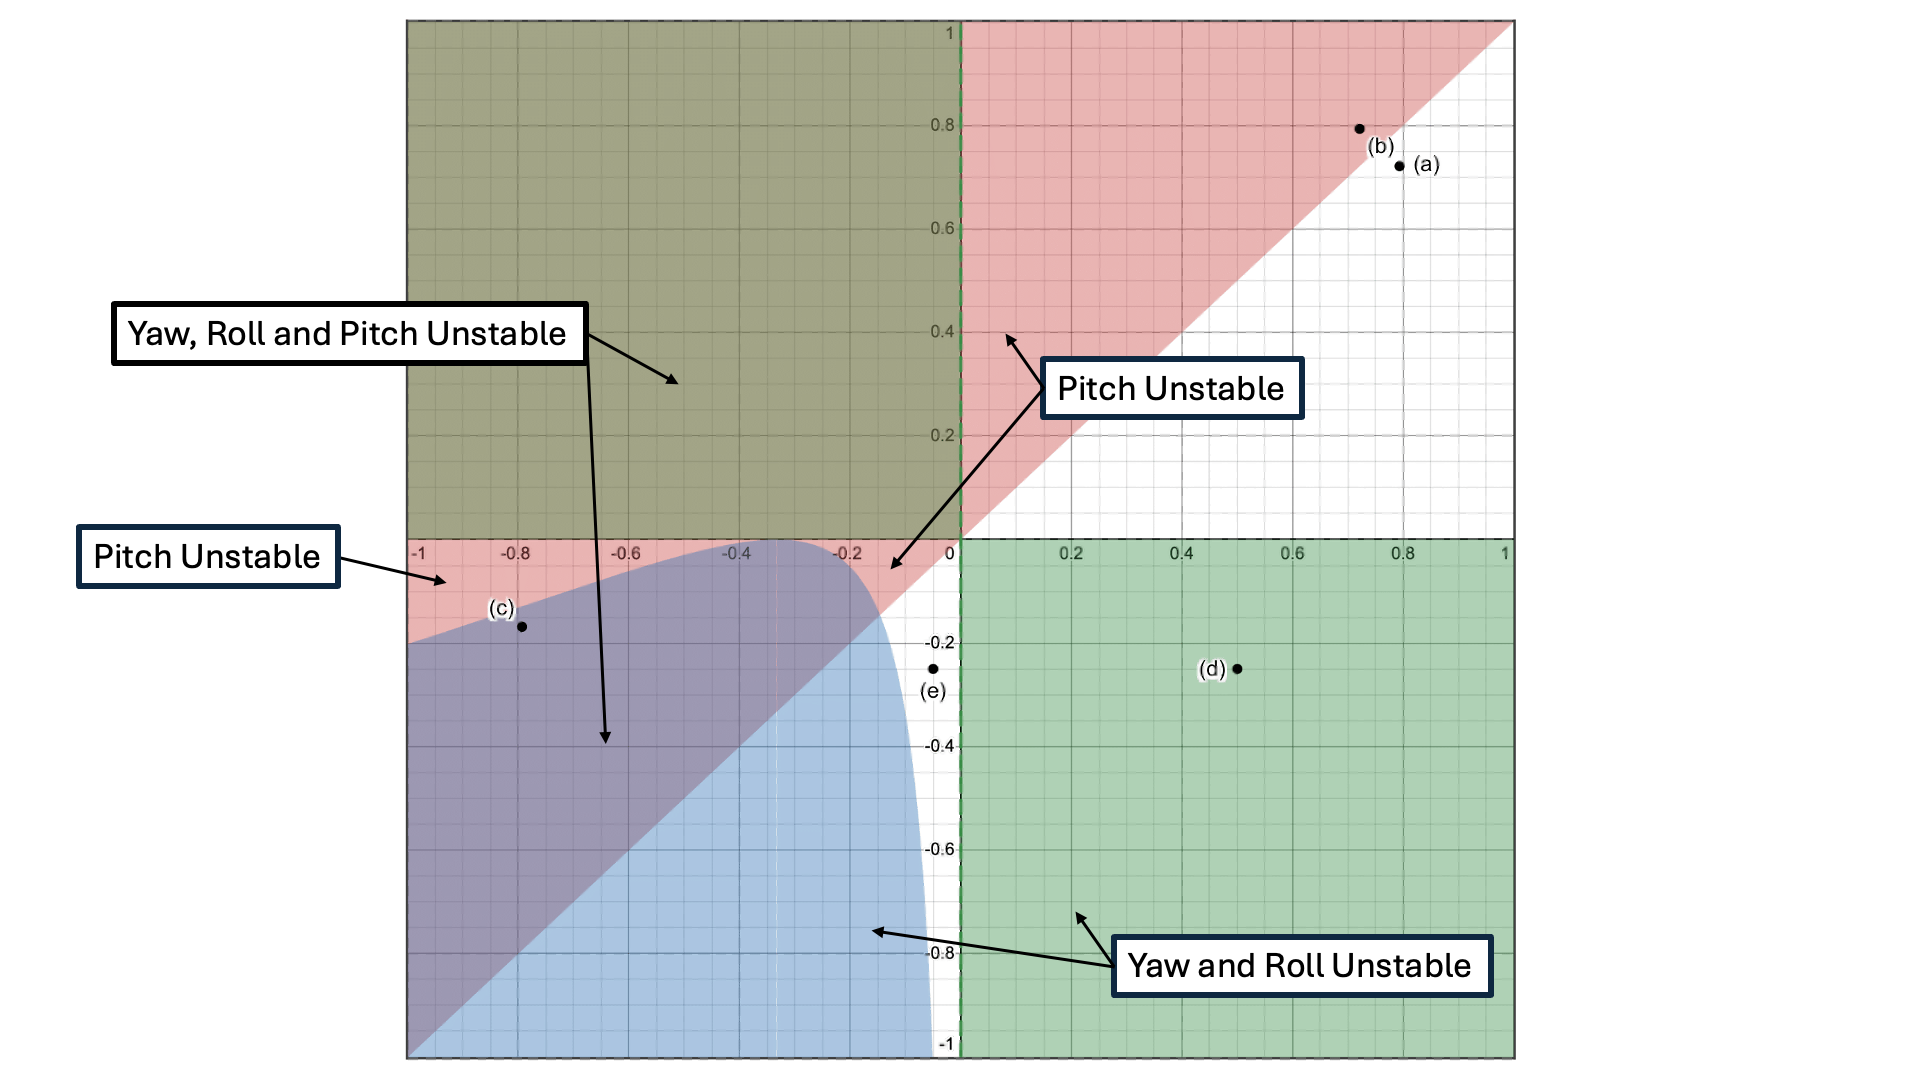
\includegraphics[width = 15cm]{Images/PS5/gravityGradientStabilityPlot.png}
    \caption{Plot of Stability Regions in the $k_Tk_R$ Plane with Various Simulated Test Points which Describe Several States of Stability and Instability}
    \label{fig:grav_gradient_stability}
\end{figure}

The definitions of $k_N$, $k_T$, and $k_R$ are seen in Equations \ref{eq:k_N}, \ref{eq:k_T}, and \ref{eq:k_R} respectively. 

\begin{eqnarray}
    k_N &= \frac{I_y - I_x}{I_z} \label{eq:k_N} \\
    k_T &= \frac{I_z - I_x}{I_y} \label{eq:k_T} \\
    k_R &= \frac{I_z - I_y}{I_x} \label{eq:k_R}
\end{eqnarray}

\subsubsection{Considering the results from 1a, comments on the expected stability of the attitude motion of your satellite about equilibrium. Try to reproduce stable and unstable motion by setting proper initial conditions and perturbing those conditions slightly (e.g., by 1\%). Plot attitude parameters (e.g., Euler angles) to show stability or instability}

There are five points indicated in Figure \ref{fig:grav_gradient_stability}, the coordinates of which are shown in Table \ref{tab:k_plane_points} along with the respective principal inertia values that yield the listed configurations.

\begin{table}[H]
    \centering
    \captionsetup{justification = centering}
    \begin{tabular}{c|ccccc}
    Point  & $k_T$ & $k_R$ & $I_{xx}$ [kg m\textsuperscript{2}] & $I_{yy}$ [kg m\textsuperscript{2}] & $I_{zz}$ [kg m\textsuperscript{2}] \\ \hline
    a &   0.7933     &   0.7212    &   17510    &   23616    &  36245 \\
    b &   0.7212     &  0.7993     &   23616    &   17510    &  36245  \\  
    c &   -0.7933     &  -0.1685     &   36245    &   23616    &  17510  \\ 
    d &   0.5000     &  -0.2500     &   16109    &   40272    &  36245  \\ 
    e &   -0.0500     &  -0.2500     &   38539    &   45879    &  36245  \\ 
    \end{tabular}
    \caption{Test Points in $k_Tk_R$ Plane for Various Stability and Instability Conditions}
    \label{tab:k_plane_points}
\end{table}

The point that corresponds to Aqua's nominal configuration is Point (a). It can be seen that this lies in a stable (unshaded) region in the first quadrant of Figure \ref{fig:grav_gradient_stability}. Initializing the simulation with the the velocities and Euler angles slightly perturbed from the equilibrium state described above, the stability can be verified in simulation. Figure \ref{fig:point_a_grav_stability} shows a time history of the velocities, the Euler angles describing rotation between the principal and RTN frames in a 312 sequence, and lastly the components of the gravity gradient induced moment expressed in the principal frame. This plot confirms the prediction that the satellite is stable, with the angular velocities all being periodically oscillating about equilibrium with a small amplitude and only slight misalignment of the principal frame from the body frame. The low magnitude of the gravity induced torque is also a good indicator that the satellite is remaining close to equilibrium.

\begin{figure}[H]
    \centering
    \captionsetup{justification = centering}
    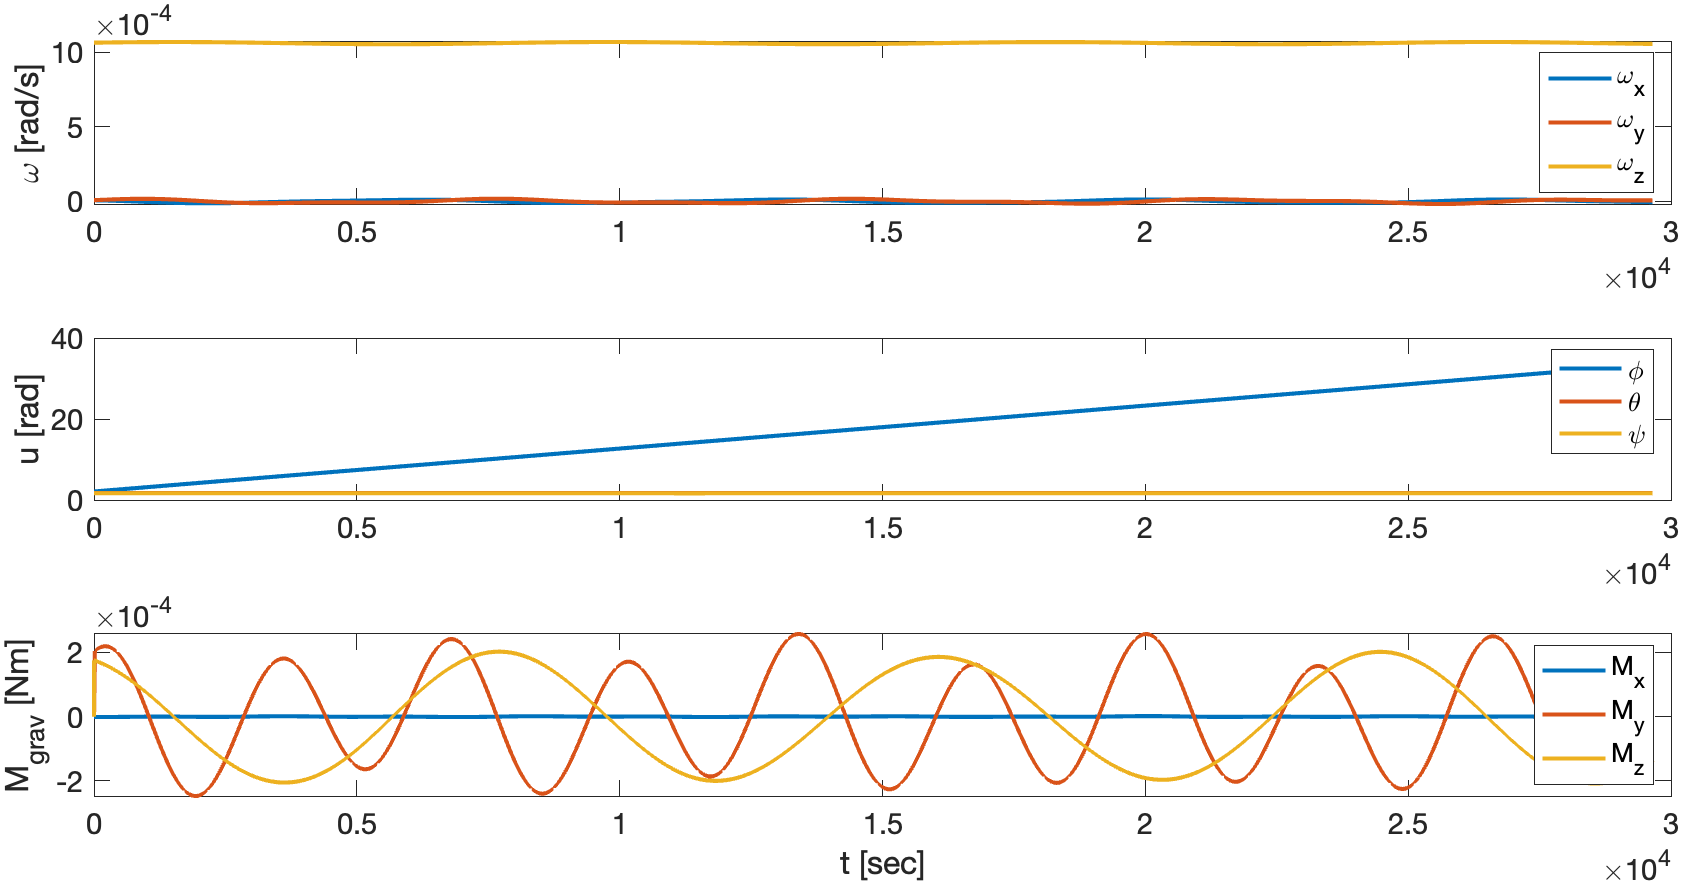
\includegraphics[width = 12cm]{Images/PS5/point_a_grav_stability.png}
    \caption{Time History of Perturbed Equilibrium for Point (a)}
    \label{fig:point_a_grav_stability}
\end{figure}

Points (b)--(d) describe unstable conditions along various axes. The following plots (Figures \ref{fig:point_b_grav_stability}--\ref{fig:point_d_grav_stability} shows the same stability analysis performed for these points.

\begin{figure}[H]
    \centering
    \captionsetup{justification = centering}
    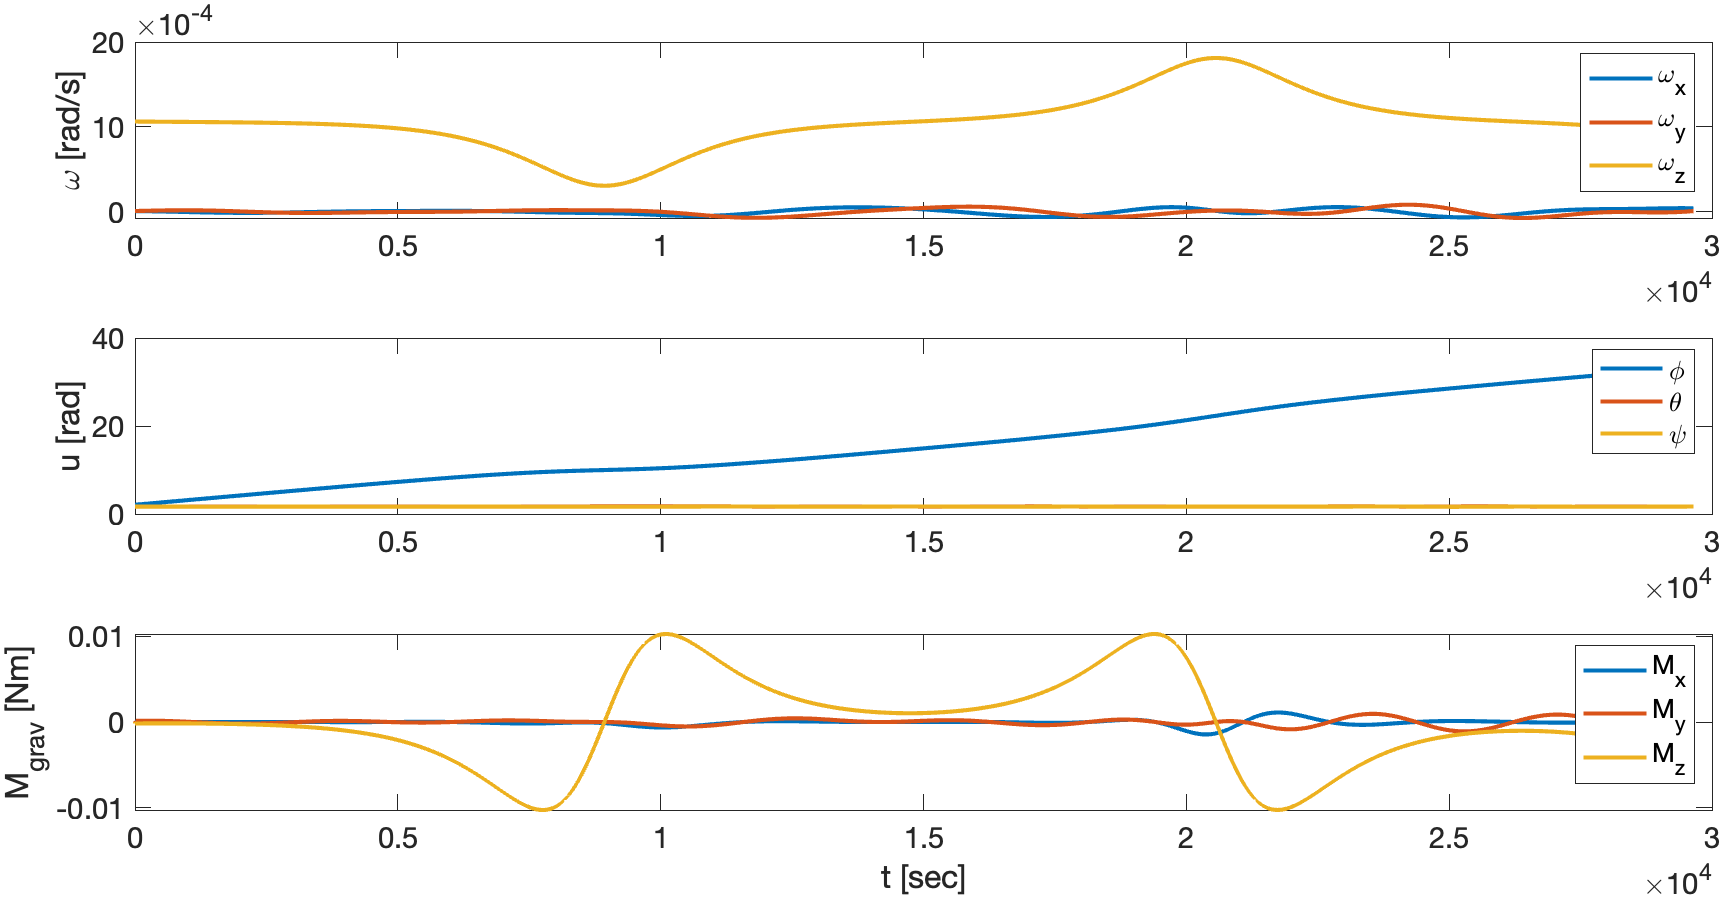
\includegraphics[width = 12cm]{Images/PS5/point_b_grav_stability.png}
    \caption{Time History of Perturbed Equilibrium for Point (b) [\emph{Pitch Unstable}]}
    \label{fig:point_b_grav_stability}
\end{figure}

\begin{figure}[H]
    \centering
    \captionsetup{justification = centering}
    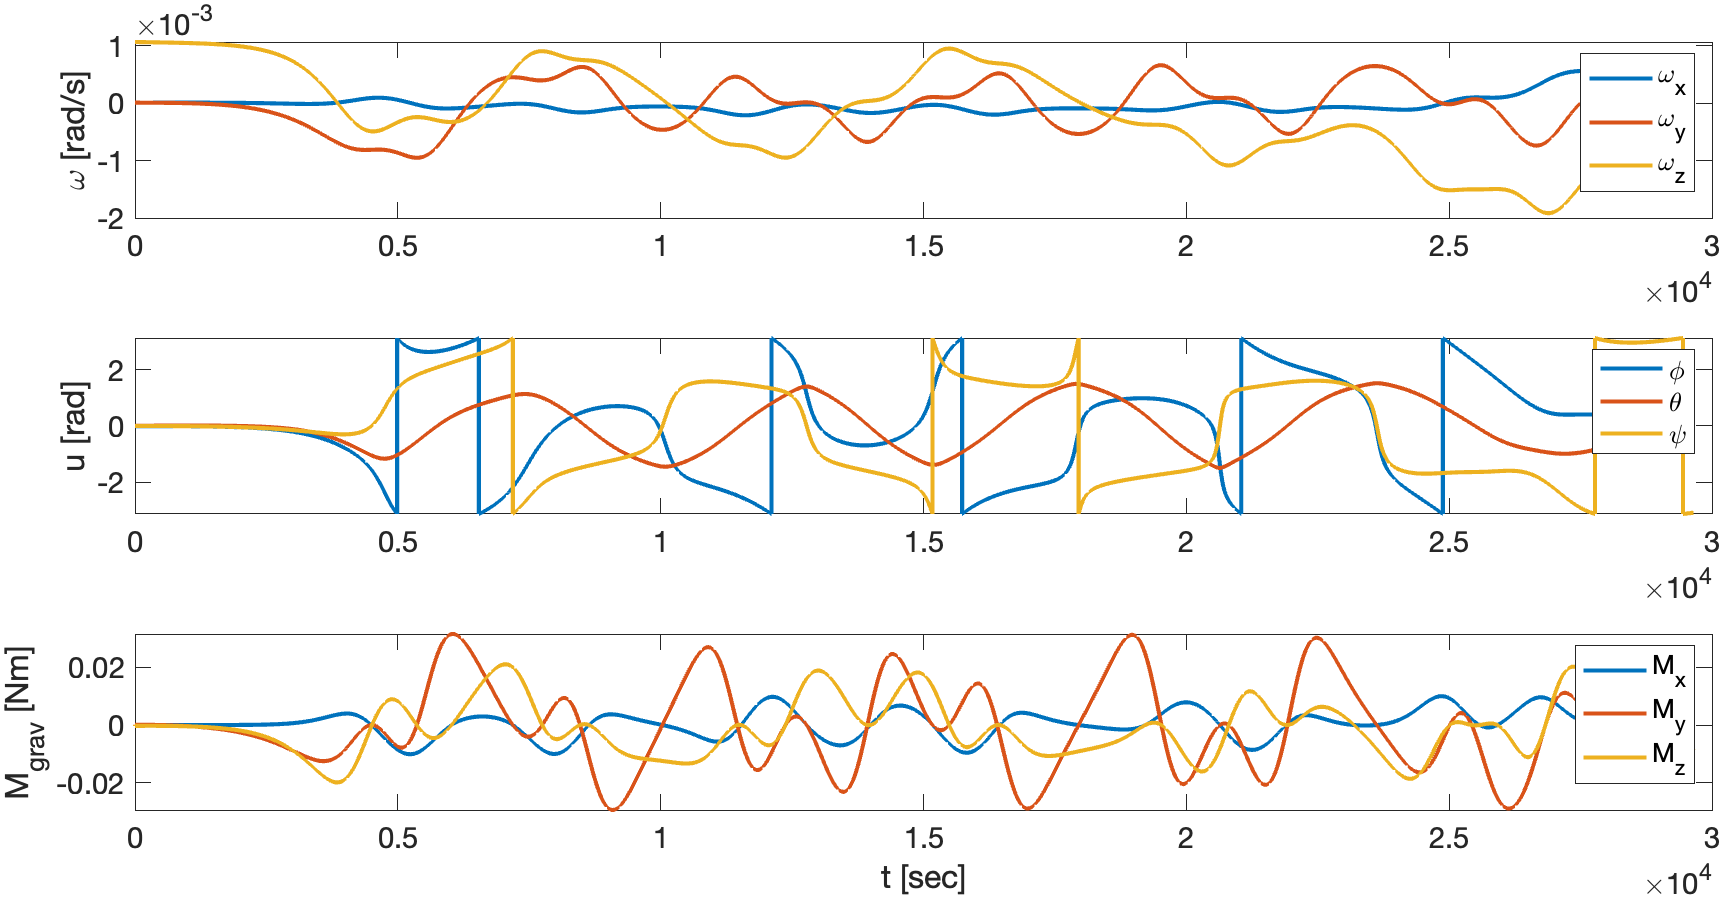
\includegraphics[width = 12cm]{Images/PS5/point_c_grav_stability.png}
    \caption{Time History of Perturbed Equilibrium for Point (c) [\emph{Roll, Yaw, and Pitch Unstable}]}
    \label{fig:point_c_grav_stability}
\end{figure}

\begin{figure}[H]
    \centering
    \captionsetup{justification = centering}
    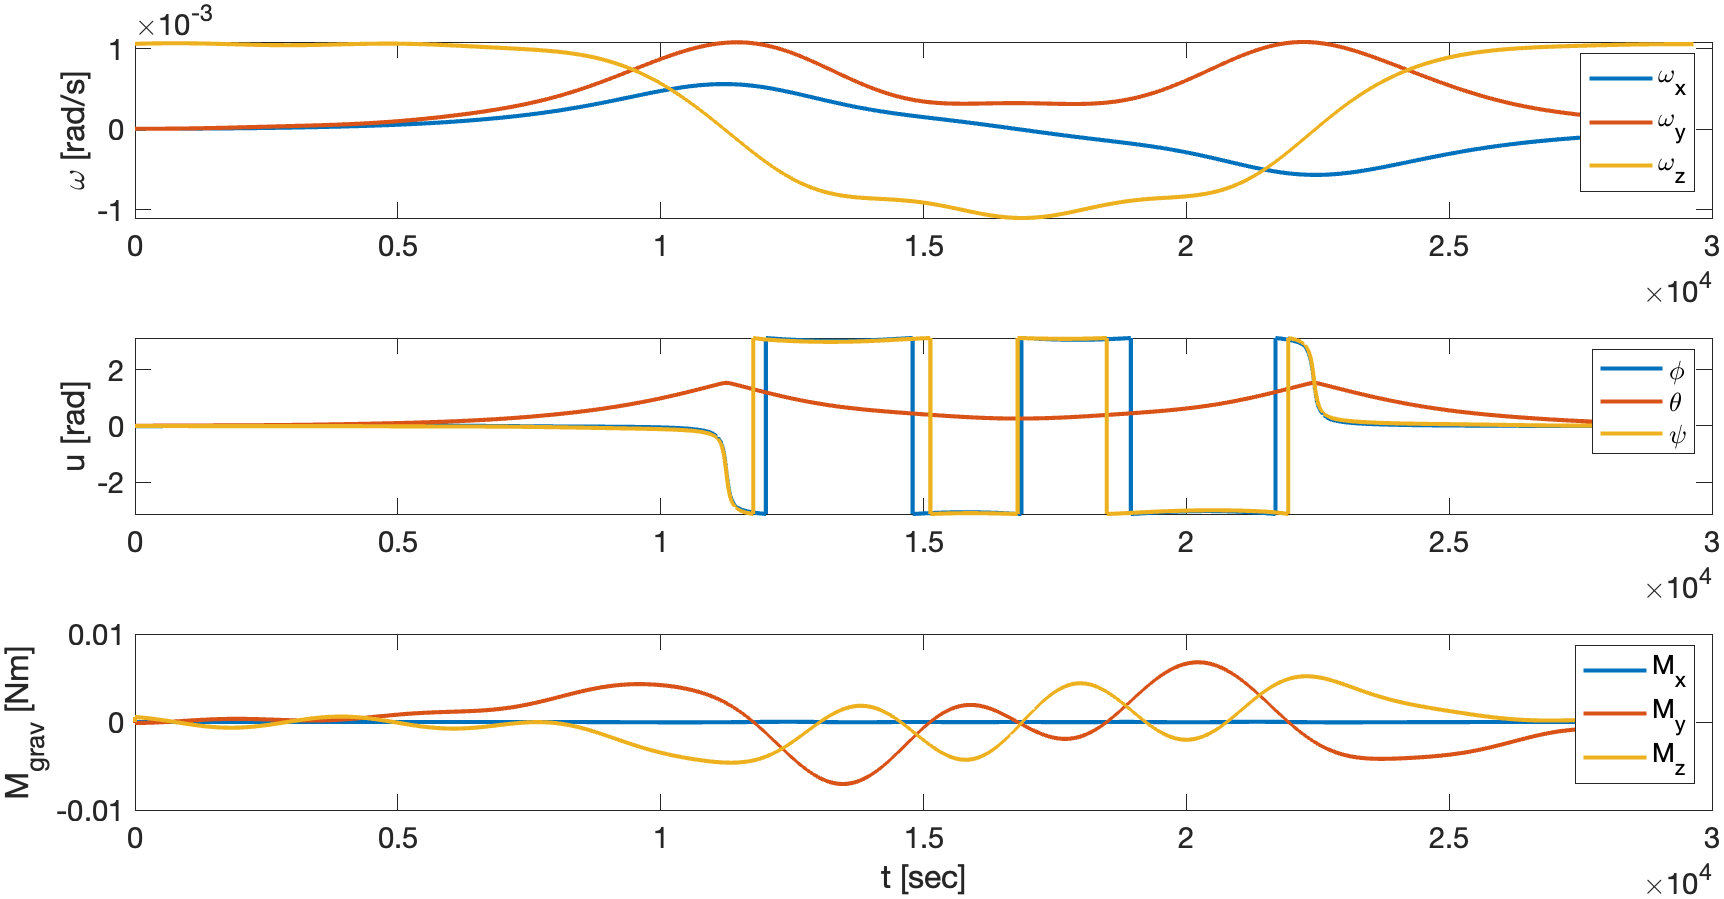
\includegraphics[width = 12cm]{Images/PS5/point_d_grav_stability.png}
    \caption{Time History of Perturbed Equilibrium for Point (d) [\emph{Roll and Yaw Unstable}]}
    \label{fig:point_d_grav_stability}
\end{figure}

Through the analysis of Figure \ref{fig:grav_gradient_stability}, Point (b) is predicted to be unstable strictly in pitch. The time history plot for this configuration show the x- and y-components of angular velocity remain periodically stable while the z-component (i.e. the pitch component) oscillates in an unstable fashion. The angle $\phi$ also deviates from 0 radians, indicating a drift away from equilibrium. Lastly the moments in the x- and y-directions stay nearly constant and close to zero while the moment in the z-direction grows.

Point (c), however, is predicted to be unstable in yaw, pitch, and roll. The simulation results clearly show all angular velocity components varying wildly in a non-periodic manner. All attitude components drift away from RTN alignment and all components of the moment vector oscillate chaotically.

Lastly, Point (d) is expected to be yaw and roll unstable while still stable in pitch. The angular velocities in the principal frame indicate that z-component swaps direction but remains nearly the same in magnitude while the x- and y-components oscillate non-periodically. The z-component of the gravity induced torque remains nearly zero as well, while the x- and y- components grow.

Another stable condition where the spacecraft is spinning about the minimum inertia is corresponds to Point (e). The stability behavior of this satellite is seen in Figure \ref{fig:point_e_grav_stability}. The time history behaves similarly for that of Point (a) as expected.

\begin{figure}[H]
    \centering
    \captionsetup{justification = centering}
    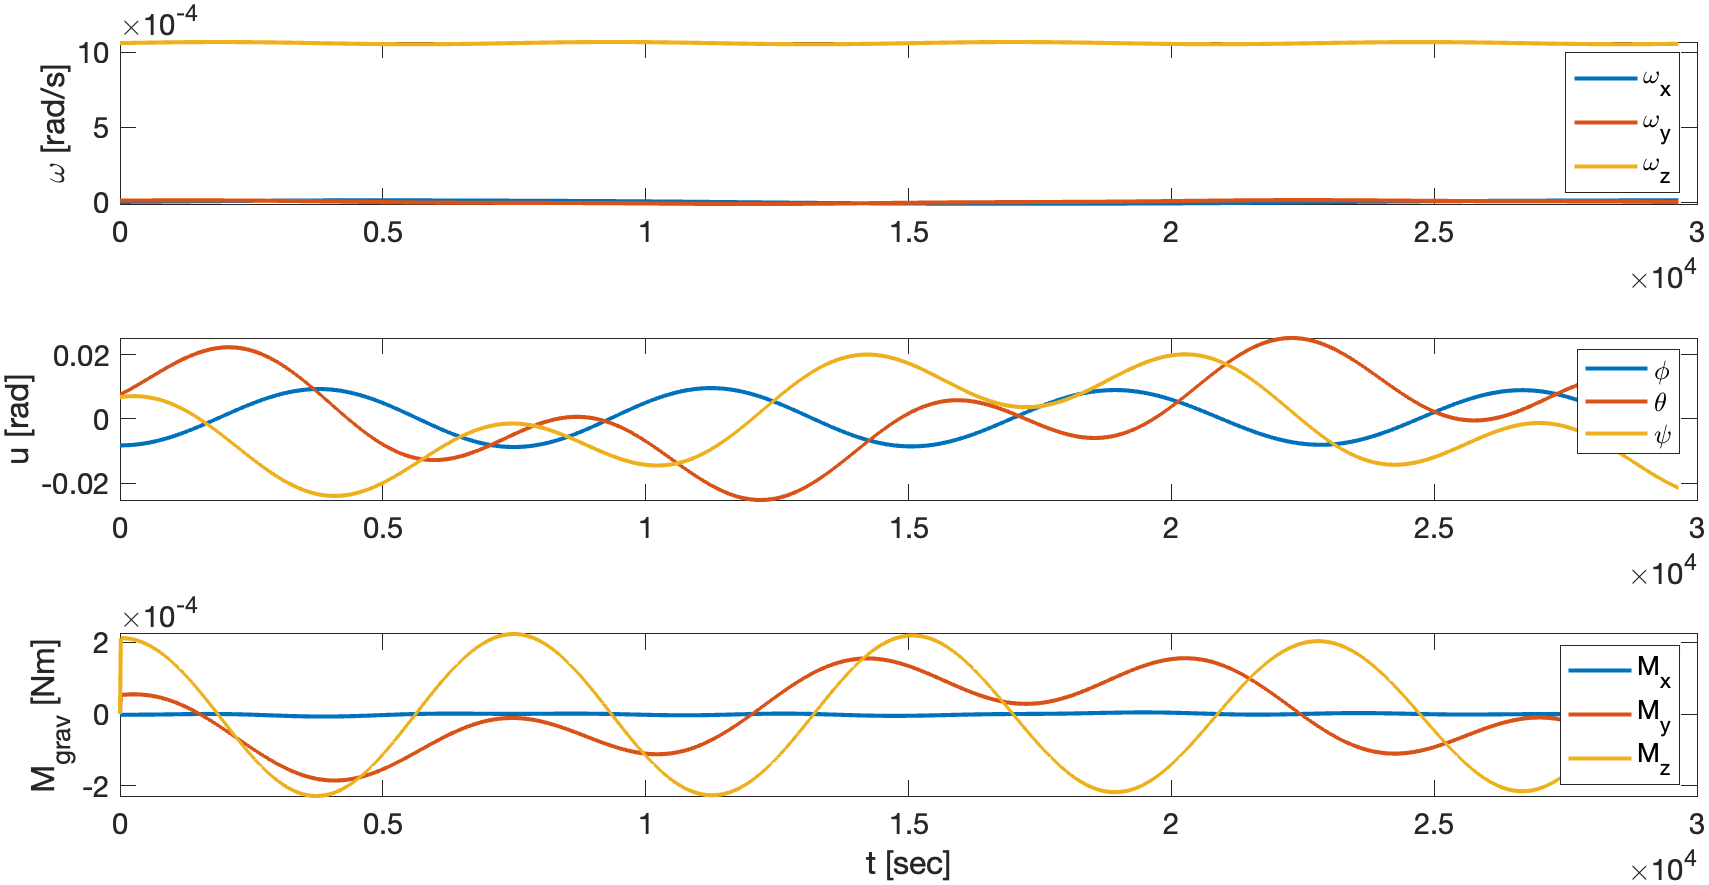
\includegraphics[width = 12cm]{Images/PS5/point_e_grav_stability.png}
    \caption{Time History of Perturbed Equilibrium for Point (e)}
    \label{fig:point_e_grav_stability}
\end{figure}

\subsubsection{How would you need to change the mass distribution and/or nominal attitude of your satellite to obtain stable motion from the gravity gradient torque? Would it make sense for your project? Show a couple of potential configurations in the Ki plane and resulting stability of attitude motion at the equilibrium. This is done by changing your inertia tensor and simulating numerically}

The spacecraft is already stable about the equilibrium described above, however it might make sense to find an equilibrium such that the spacecraft is spinning about its minimum inertia. This would ensure that the craft was already in its lowest energy state, so any unmodeled dissipation would not result in the orientation of the spacecraft changing. Very fortunately, the minimum axis of inertia for the nominal Aqua model (i.e. the x-axis in the current principal frame) is closely aligned with the y-axis in the body frame. An Earth pointing orientation for this mission is synonymous with this axis being aligned with the N-axis in the RTN frame. Therefore, it would make sense to achieve stable equilibrium about this axis. The stability of the spacecraft in this orientation will be investigated in the future.

\subsection{In addition to gravity gradient, start programming perturbation torques due to magnetic field, solar radiation pressure, and atmospheric drag.}

\subsubsection{Magnetic Field}

To create a simple, early use model for the magnetic disturbance torques, the Earth is modeled as a magnetic dipole. This assumption is not accurate for LEO, but will give helpful insight to how the spacecraft motion will be affected by this disturbance along with the ability to size actuators. A more accurate model will be investigated in the future. The dipole model for the Earth is given by Equation \ref{eq:earth_mag_field} where $R_E$ is the radius of the earth (6371.8 km), $B_0$ is the strength of Earth's magnetic field at the surface (30800 nT), $\vec{R} = R \hat{R}$ is the vector from the center of the Earth to the center of mass of the spacecraft, and $\hat{m}$ represents the direction of Earth's magnetic dipole.

\begin{equation} \label{eq:earth_mag_field}
    \vec{B}(\vec{R}) = -\frac{R_E^3 B_0}{R^3} \left[ 3\left( \hat{m} \cdot \hat{R} \right) - \hat{m} \right]
\end{equation}

When modeling the magnetic dipole of the spacecraft, a major simplification was made. The spacecraft was split into two main components---the chassis along and instruments as one component with the solar panel as another. Each component is modeled as a insulating cylinder with an electromagnetic coil wrapped around it. The model for the dipole moment created by each of these components is described in Equation \ref{eq:spacecraft_dipole}, where $\mu_0$ is the permeability of vacuum (1.25663706212 $\times$ 10 \textsuperscript{-9} N A \textsuperscript{-2}), S is the surface area between each coil, $n$ is the number of coils, and $\Delta I$ is the variable current passing through the coil. For the current state of the model, these numbers were chosen very arbitrarily. They are reported in Table \ref{tab:spacecraft_dipole_data} along with the direction in the body frame and magnitude of the resulting dipole moment.

\begin{equation} \label{eq:spacecraft_dipole}
    \vec{m} = \mu_0 S n \Delta I \hat{m}
\end{equation}

\begin{table}[H]
    \centering
    \captionsetup{justification = centering}
    \begin{tabular}{c|ccccc}
    Component  & S [m\textsuperscript{2}] & $n$ & $\Delta I$ [A] & $\hat{m}$  & m [$10^{-4}$ Nm/T] \\ \hline
    Chassis + Instruments &   3     &   15    &   1    &   $\begin{bmatrix}  1 & 0 & 0  \end{bmatrix}^T$    &  0.5655 \\
    Solar Panel &   0.2     &  15    &   1    &    $\begin{bmatrix}  0 & 1 & 0  \end{bmatrix}^T$   &  0.0377  \\  
    \end{tabular}
    \caption{Heuristics used for Spacecraft Dipole Moment Modeling}
    \label{tab:spacecraft_dipole_data}
\end{table}

This approximation of the disturbance was implemented using the Simulink model depicted in Figure \ref{fig:simulink_mag}.

\begin{figure}[H]
    \centering
    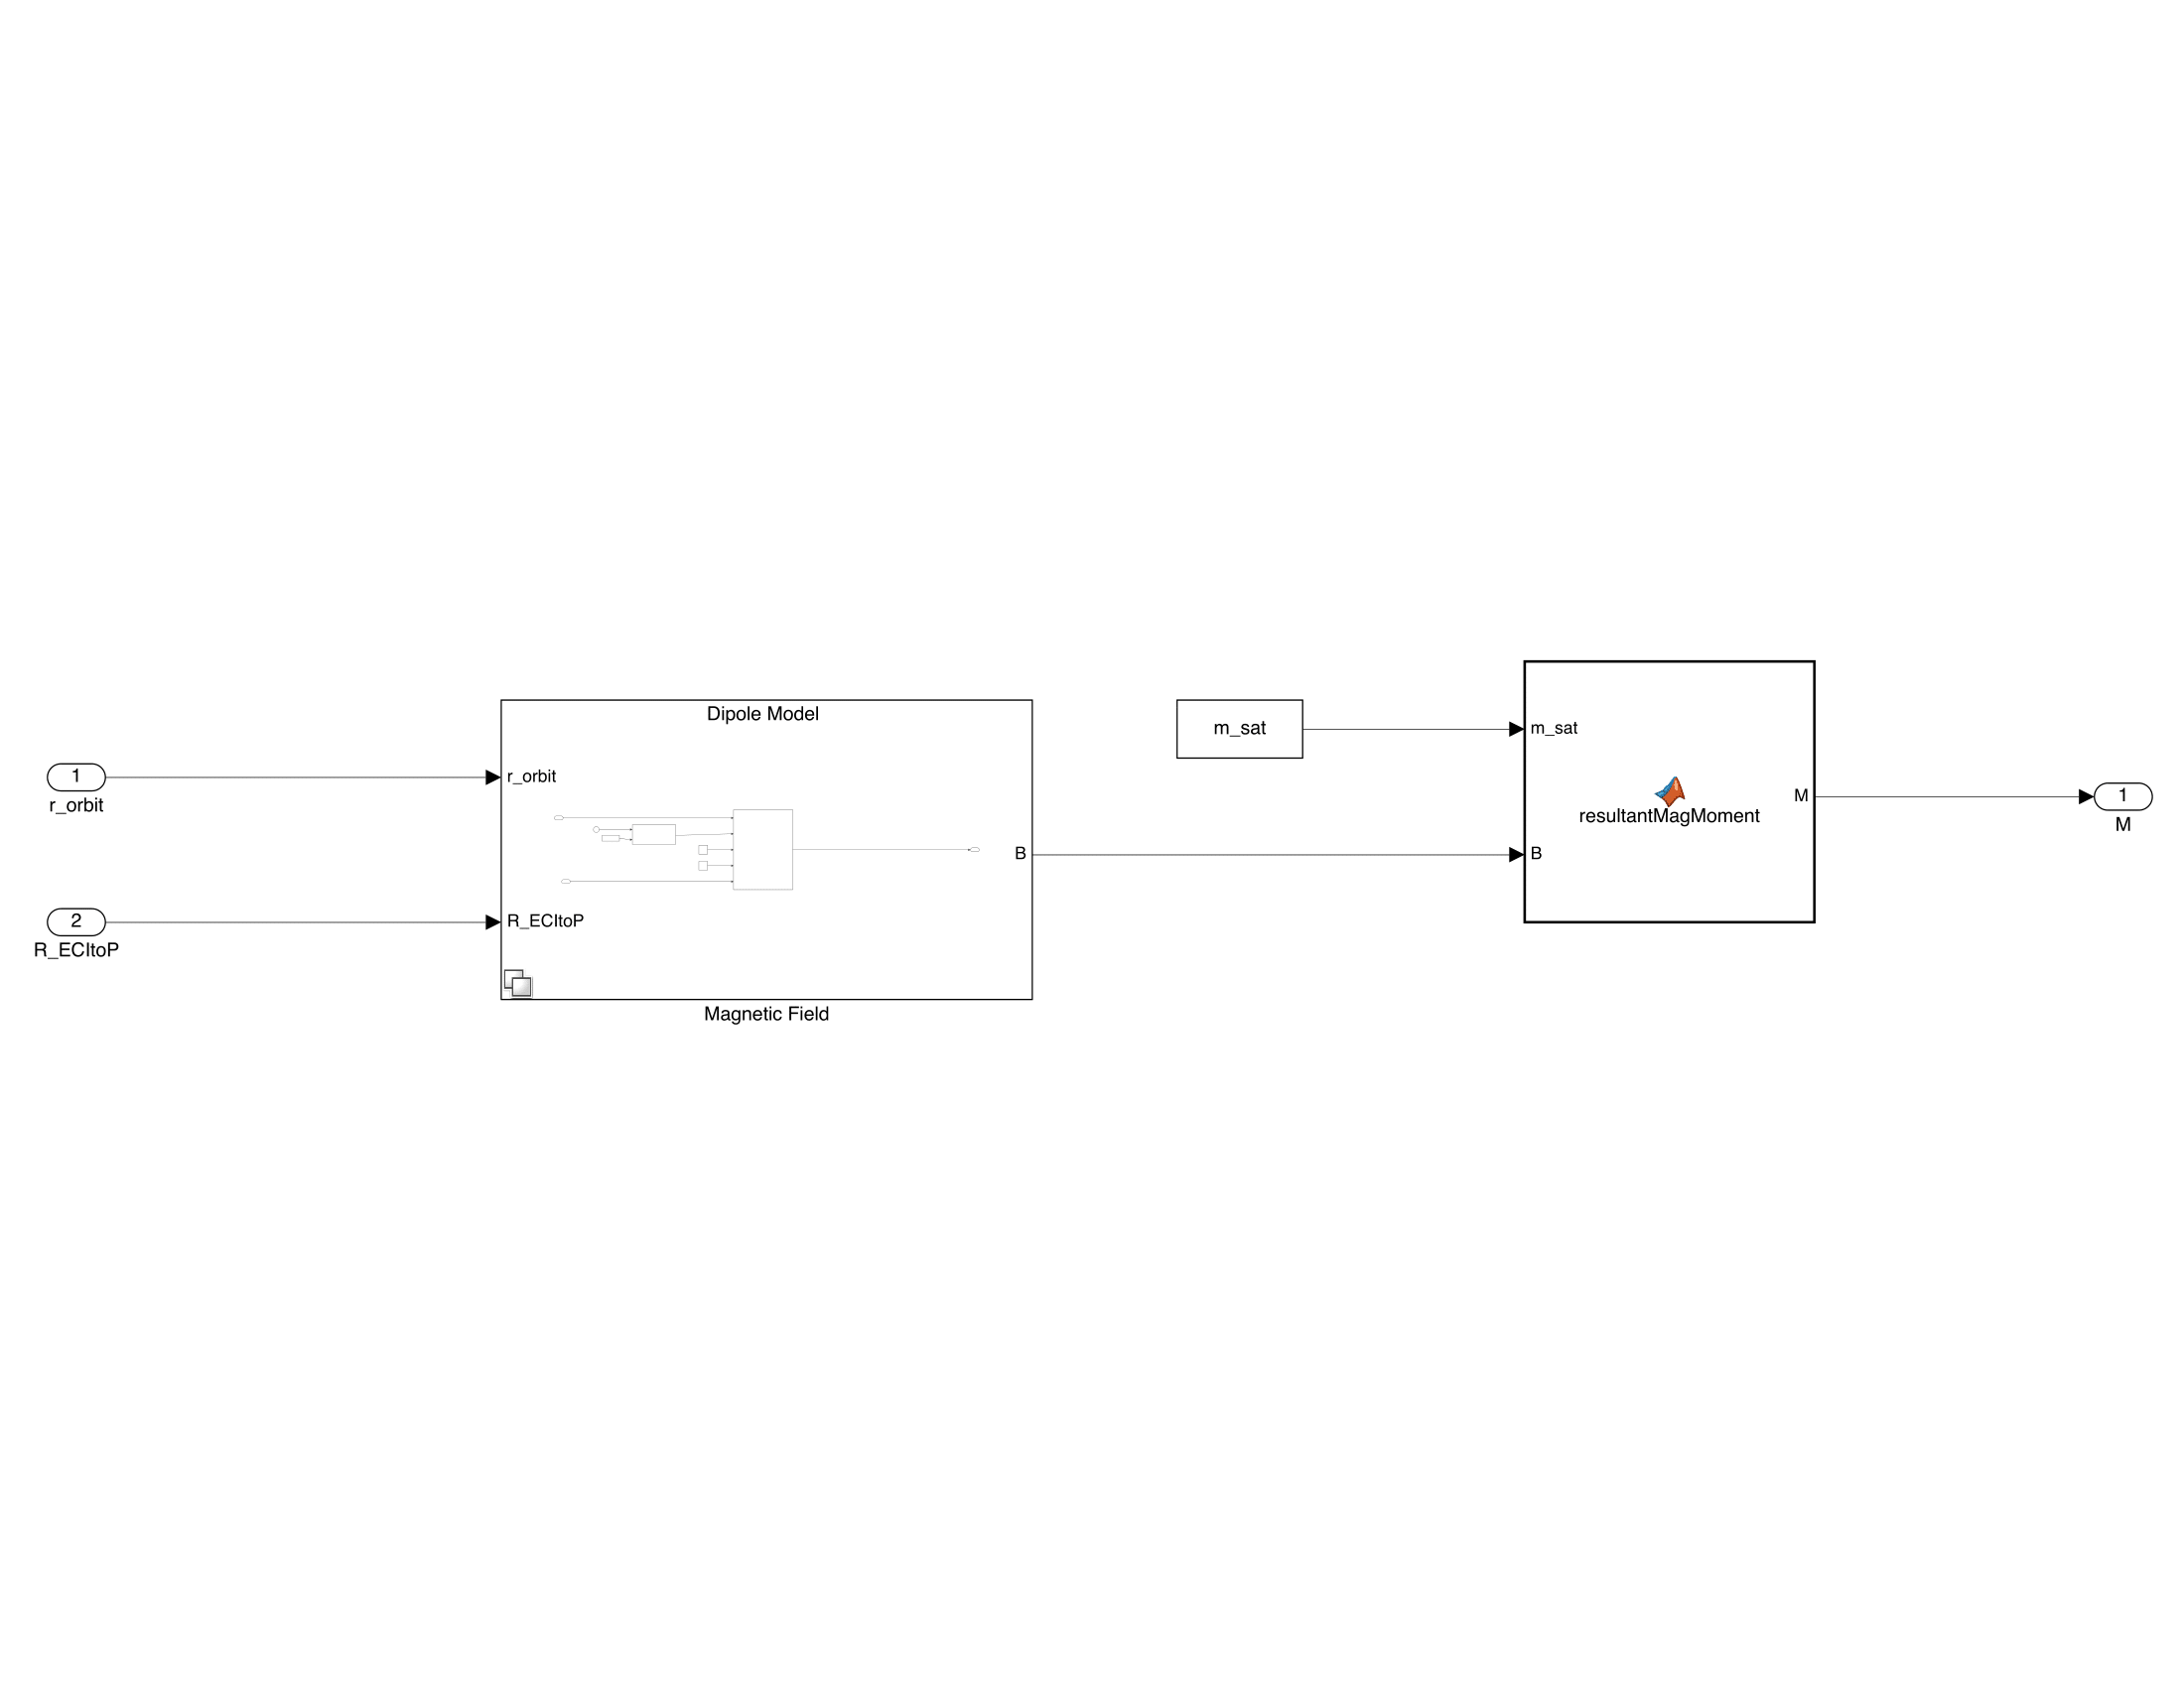
\includegraphics[trim={0.25cm 6cm 0.25cm 6cm},clip,width = 15cm]{Images/PS5/magneticField-1.png}
\end{figure}

\begin{figure}[H]
    \centering
    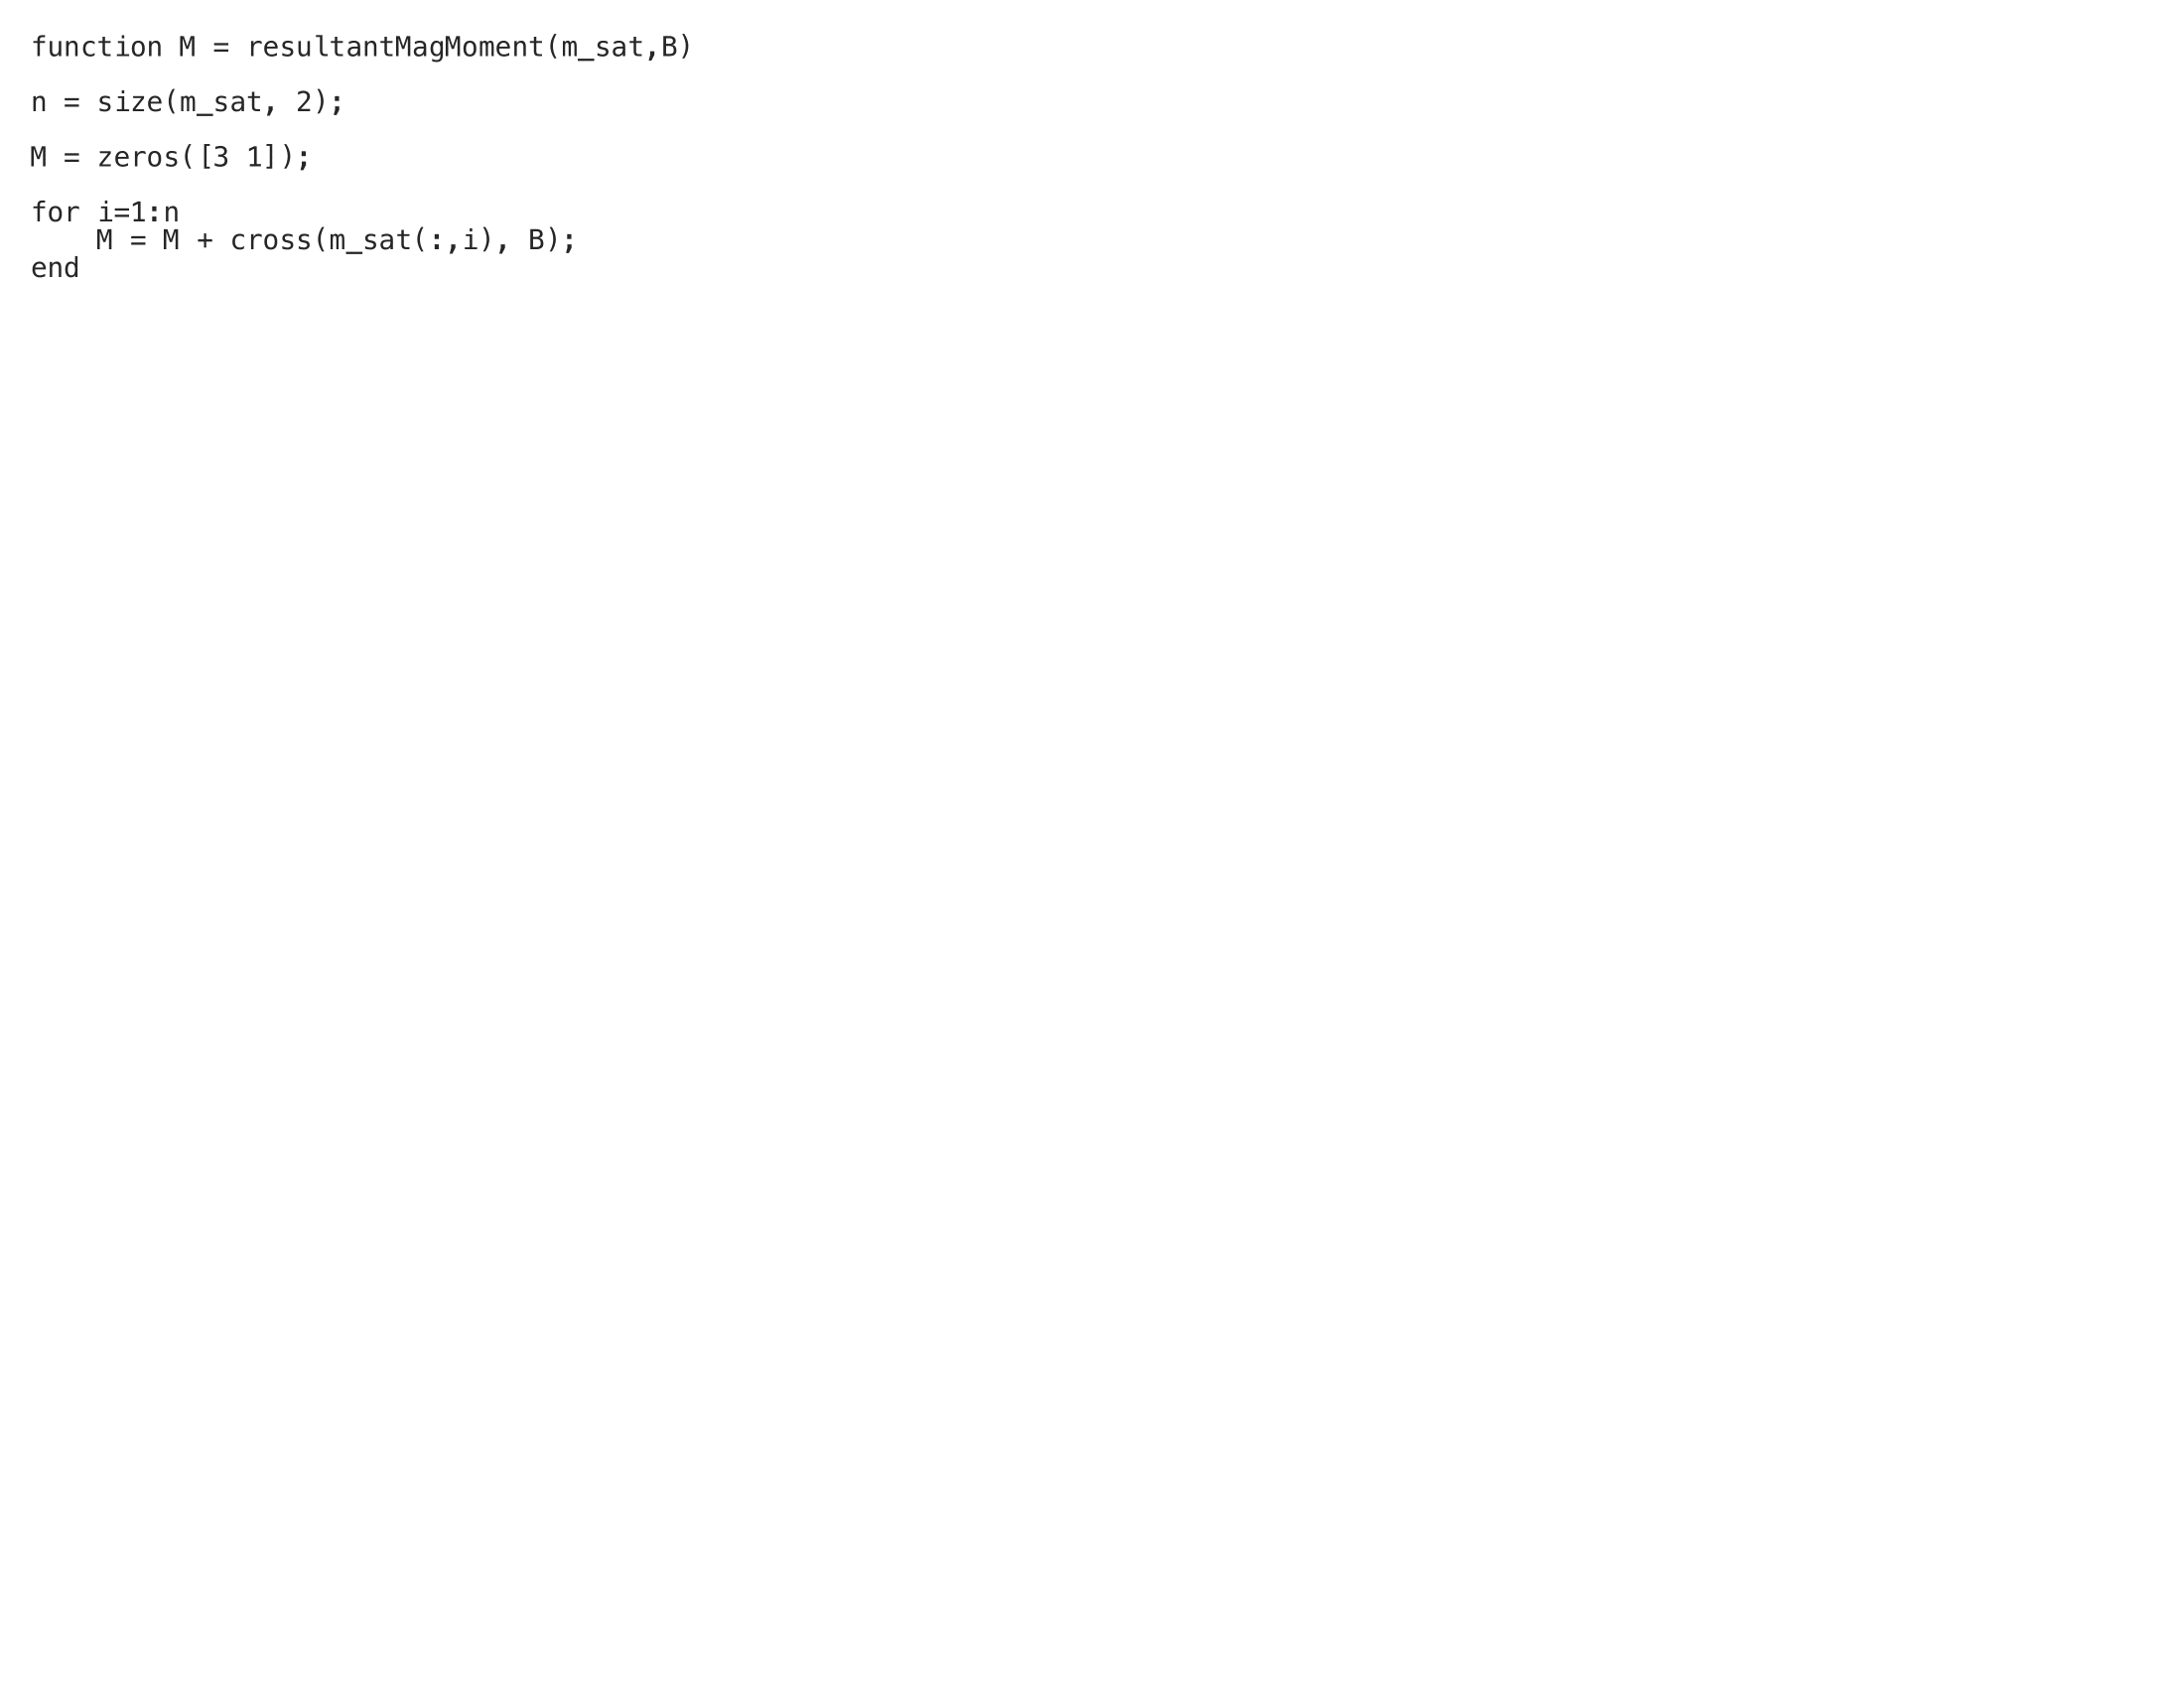
\includegraphics[trim={0cm 18cm 18cm 0cm},clip,width = 10cm]{Images/PS5/magneticField-2.png}
\end{figure}

\begin{figure}[H]
    \centering
    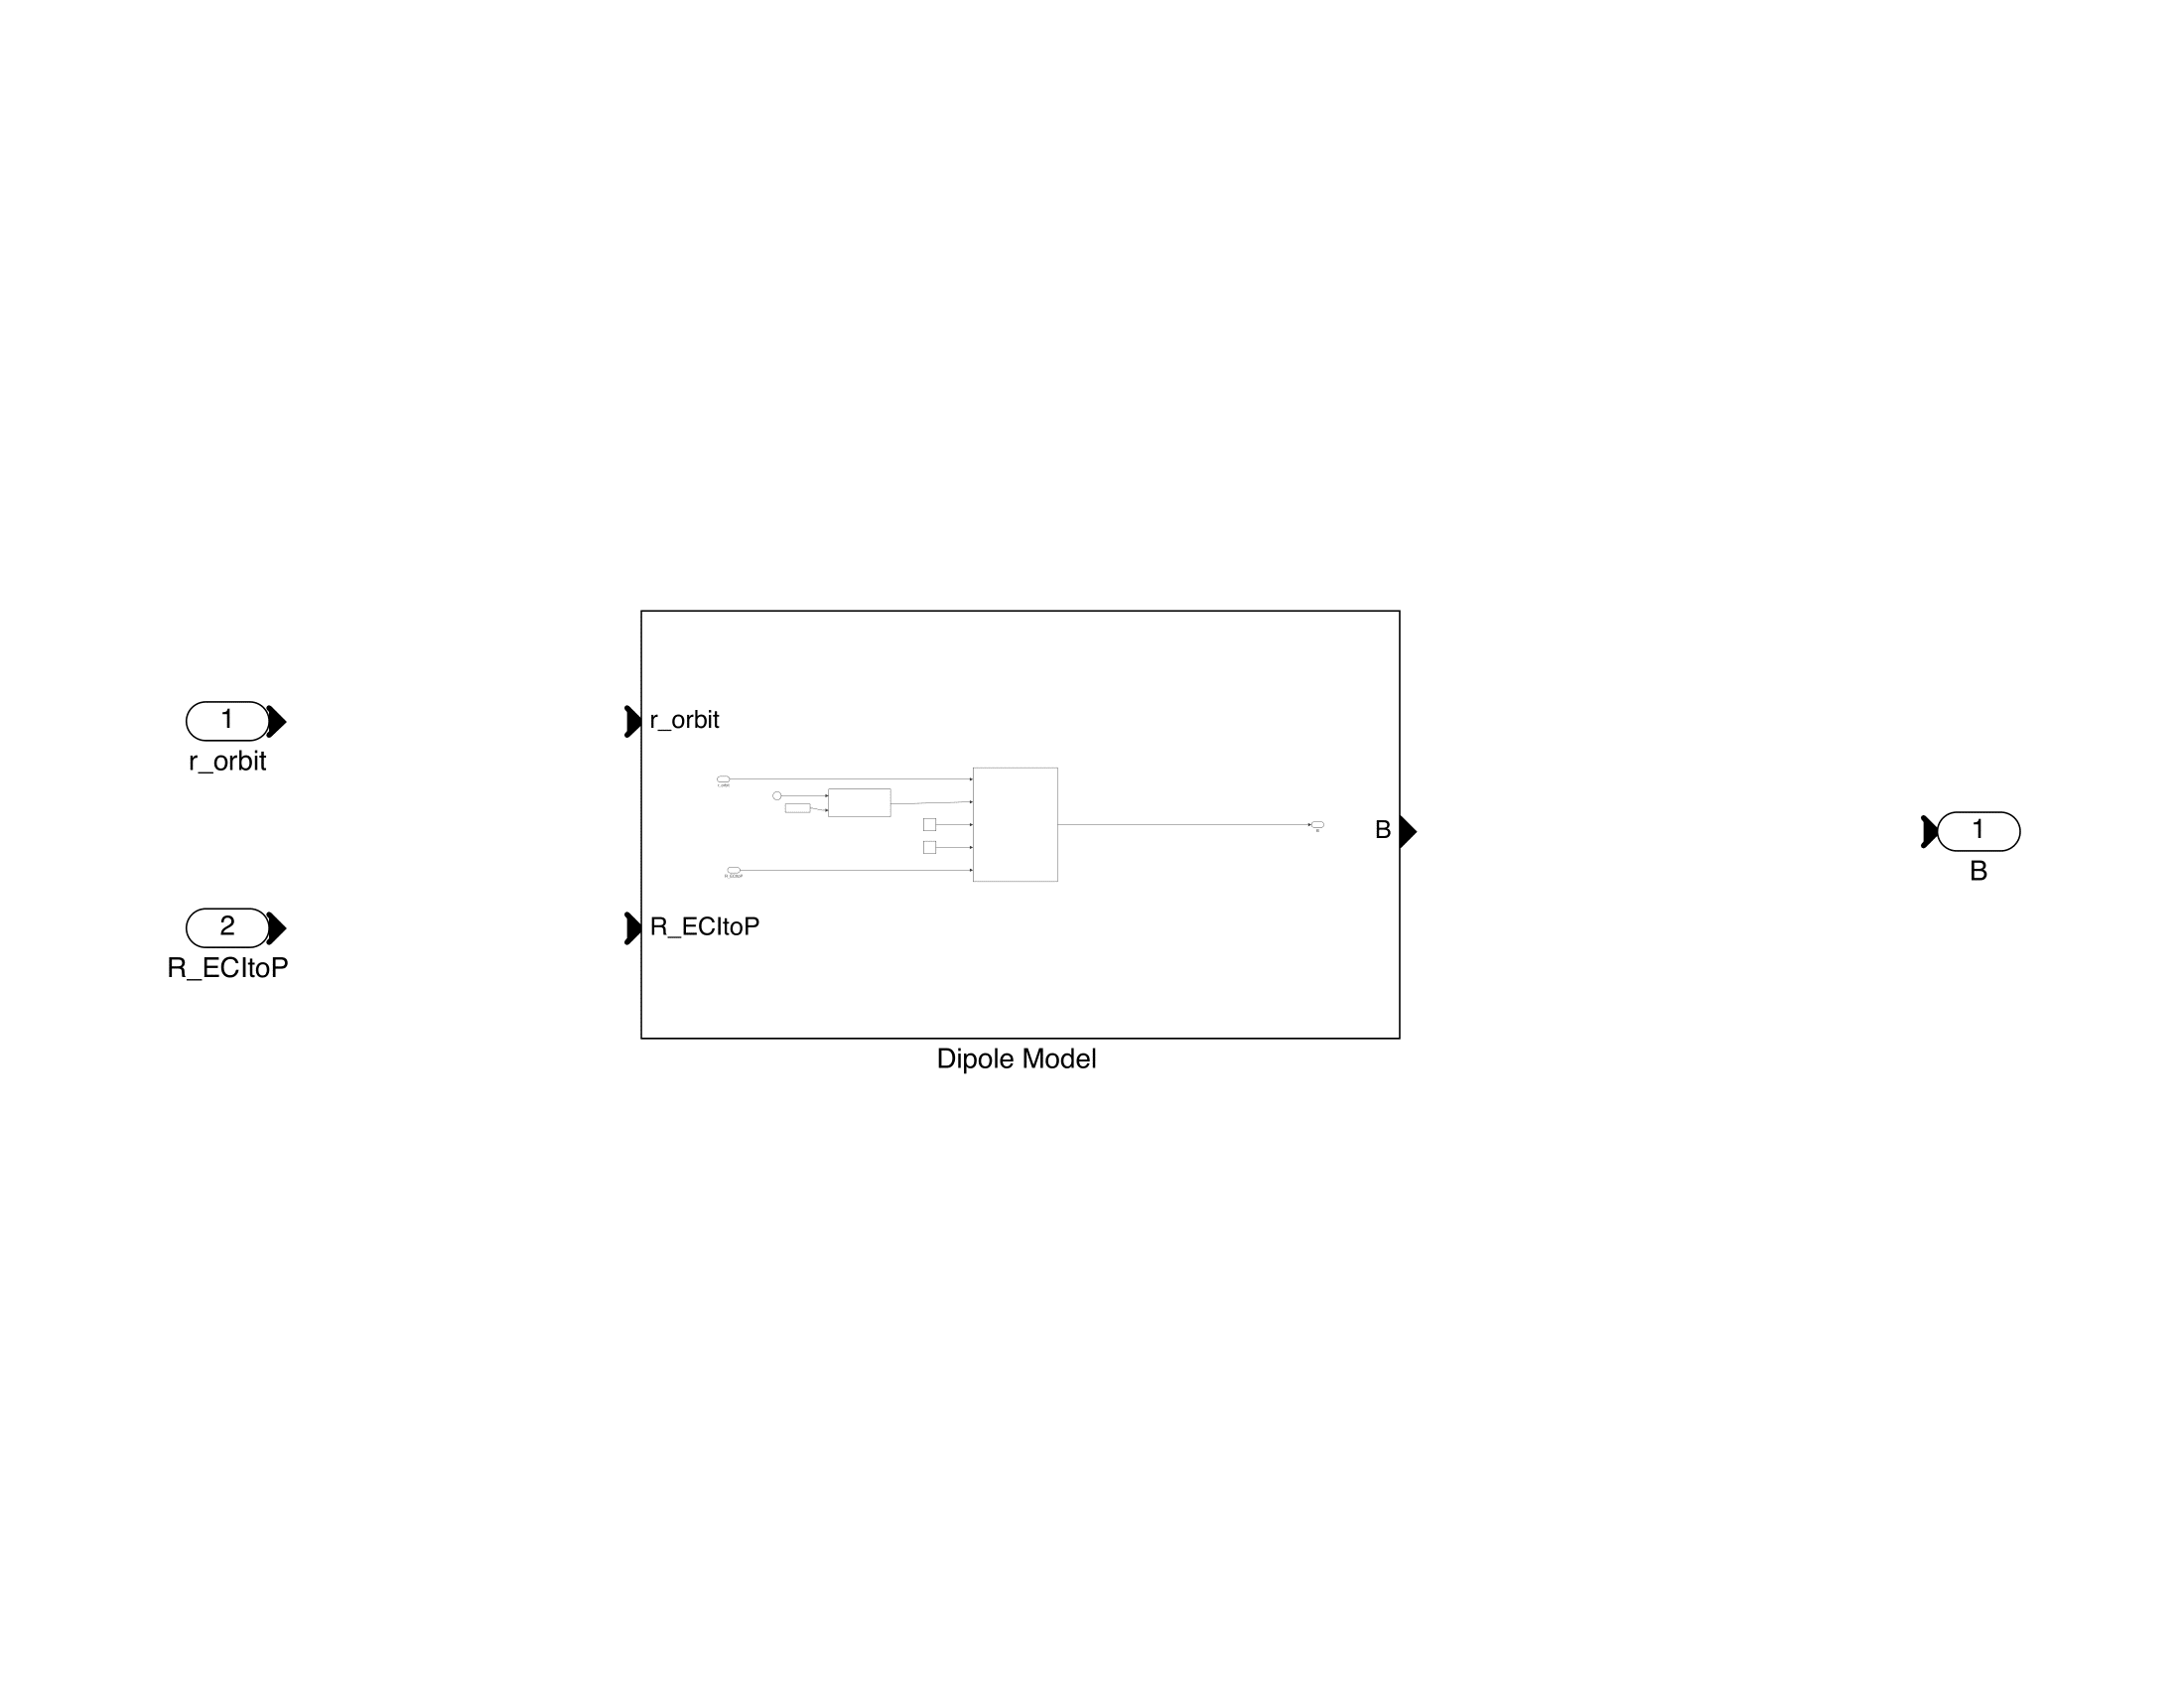
\includegraphics[trim={0.25cm 6cm 0.25cm 6cm},clip,width = 15cm]{Images/PS5/magneticField-3.png}
\end{figure}

\begin{figure}[H]
    \centering
    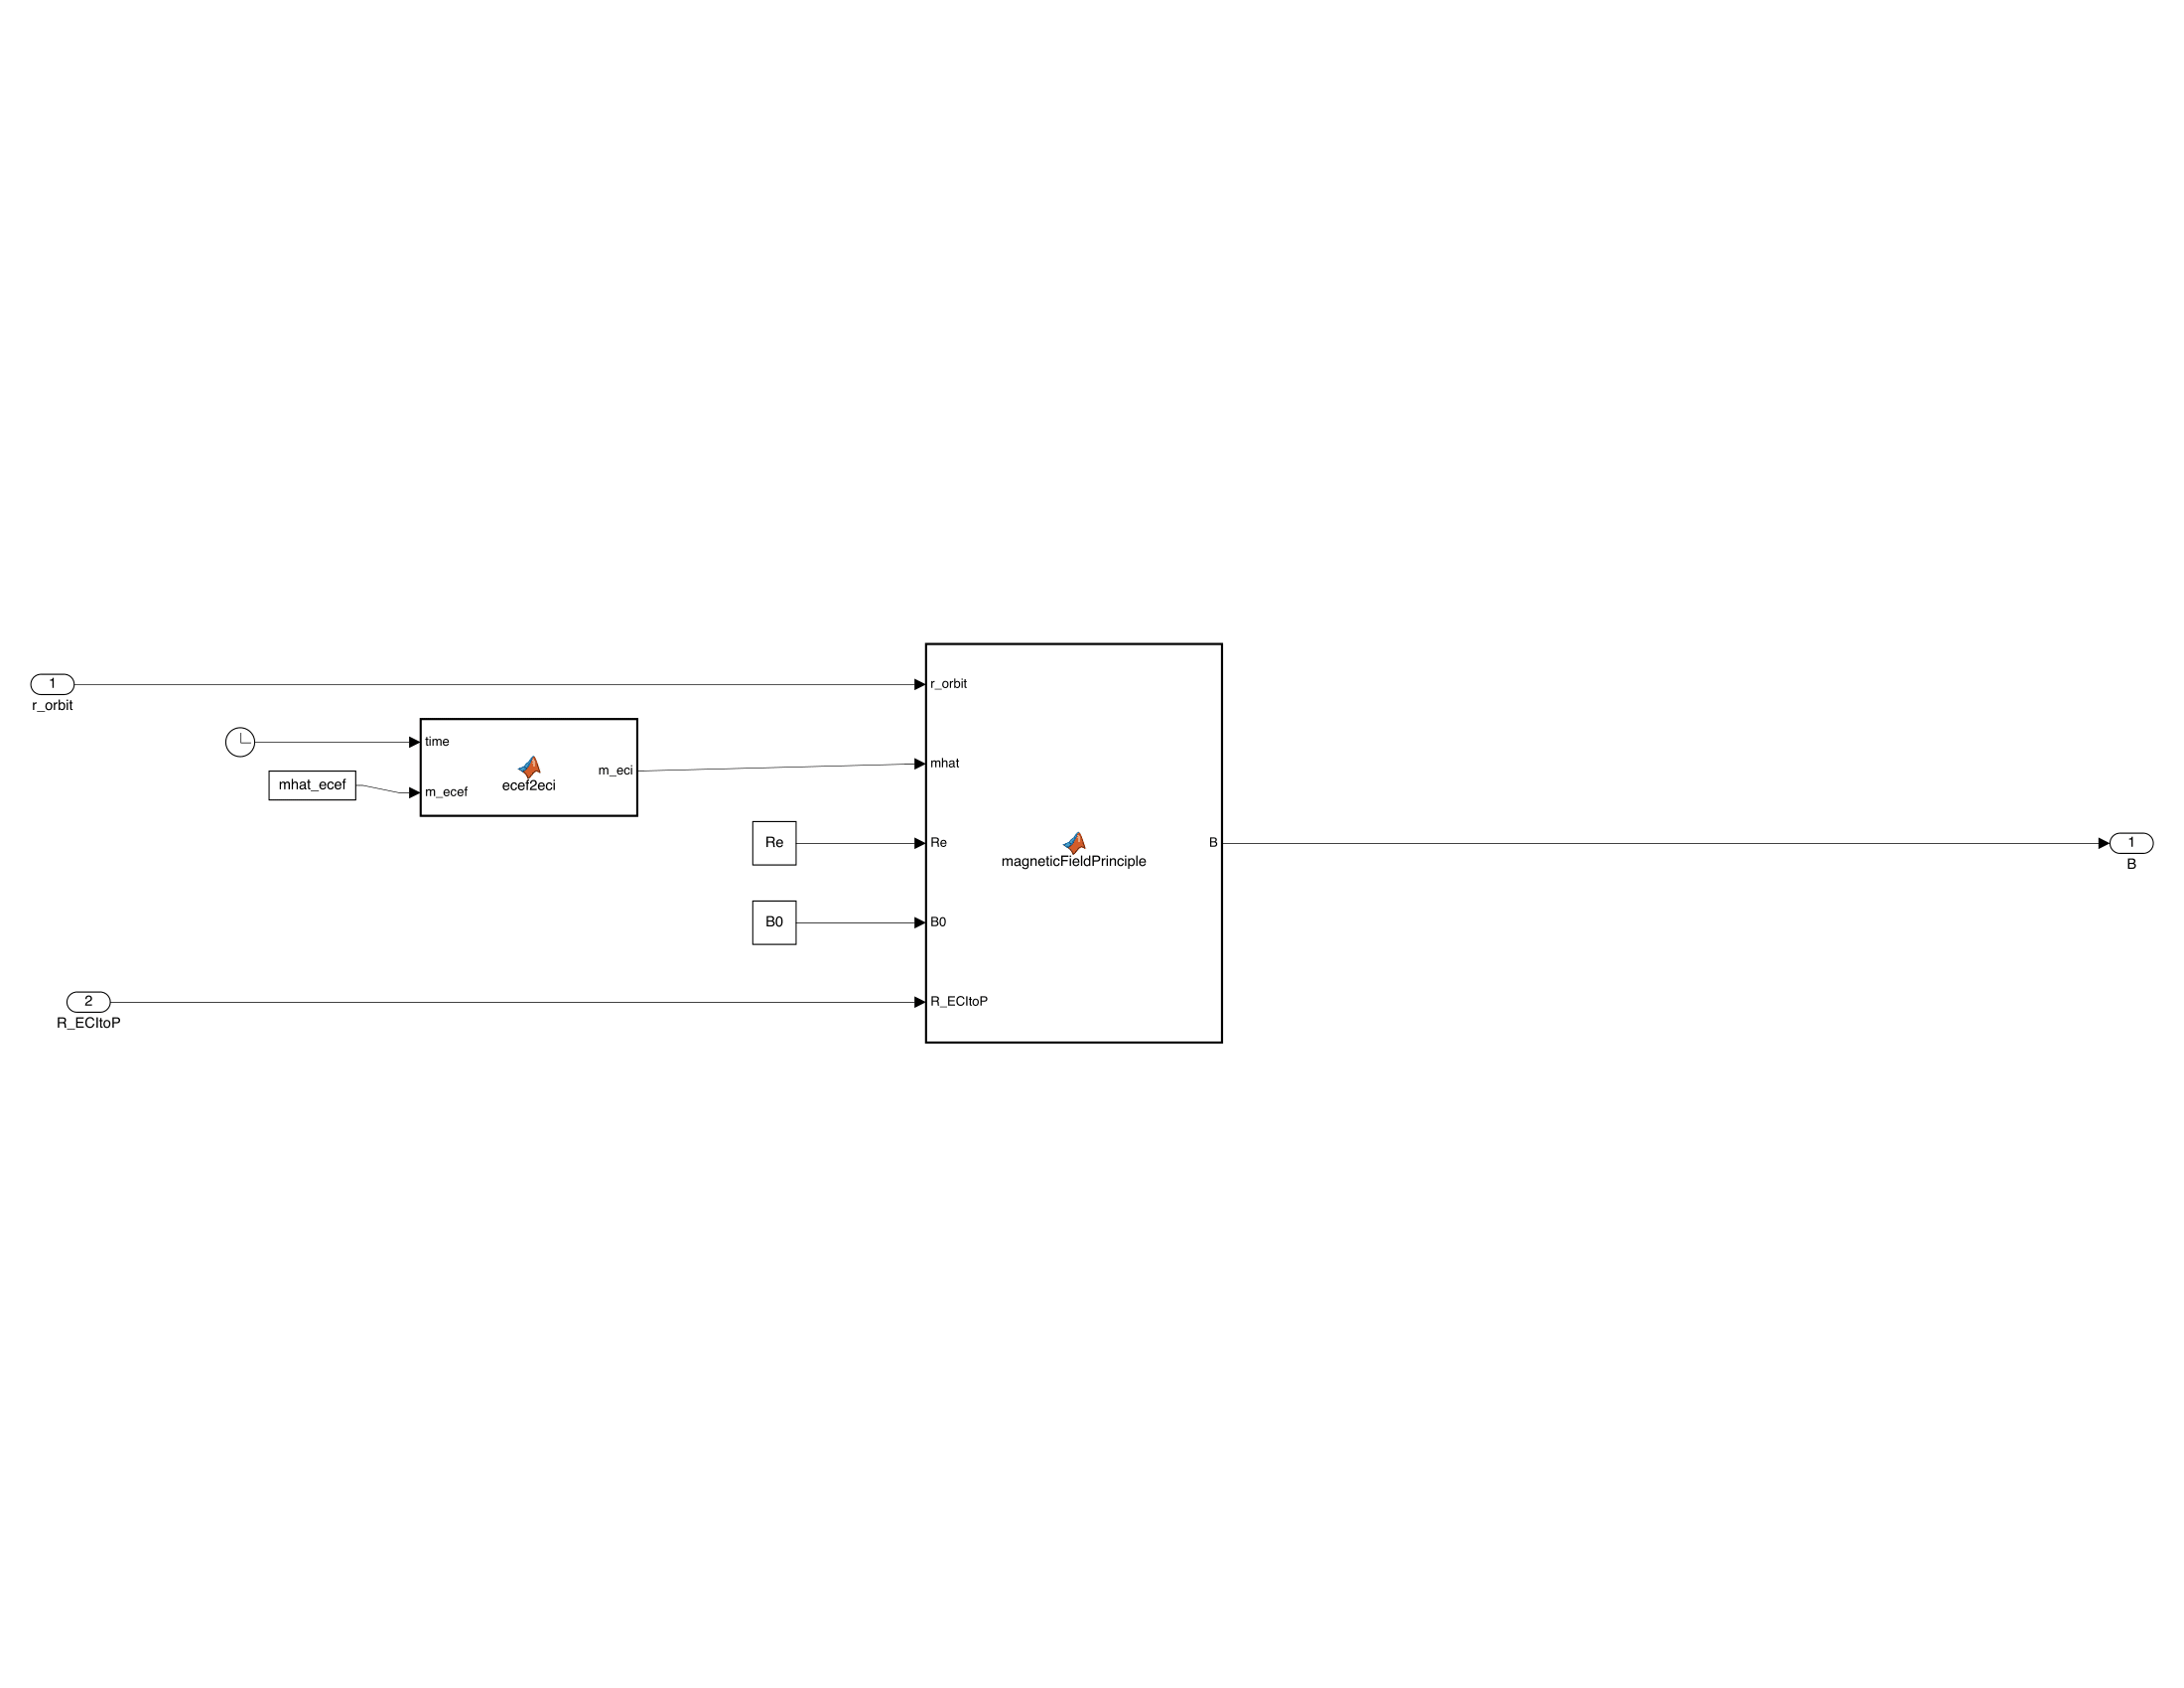
\includegraphics[trim={0.25cm 6cm 0.25cm 6cm},clip,width = 15cm]{Images/PS5/magneticField-4.png}
\end{figure}

\begin{figure}[H]
    \centering
    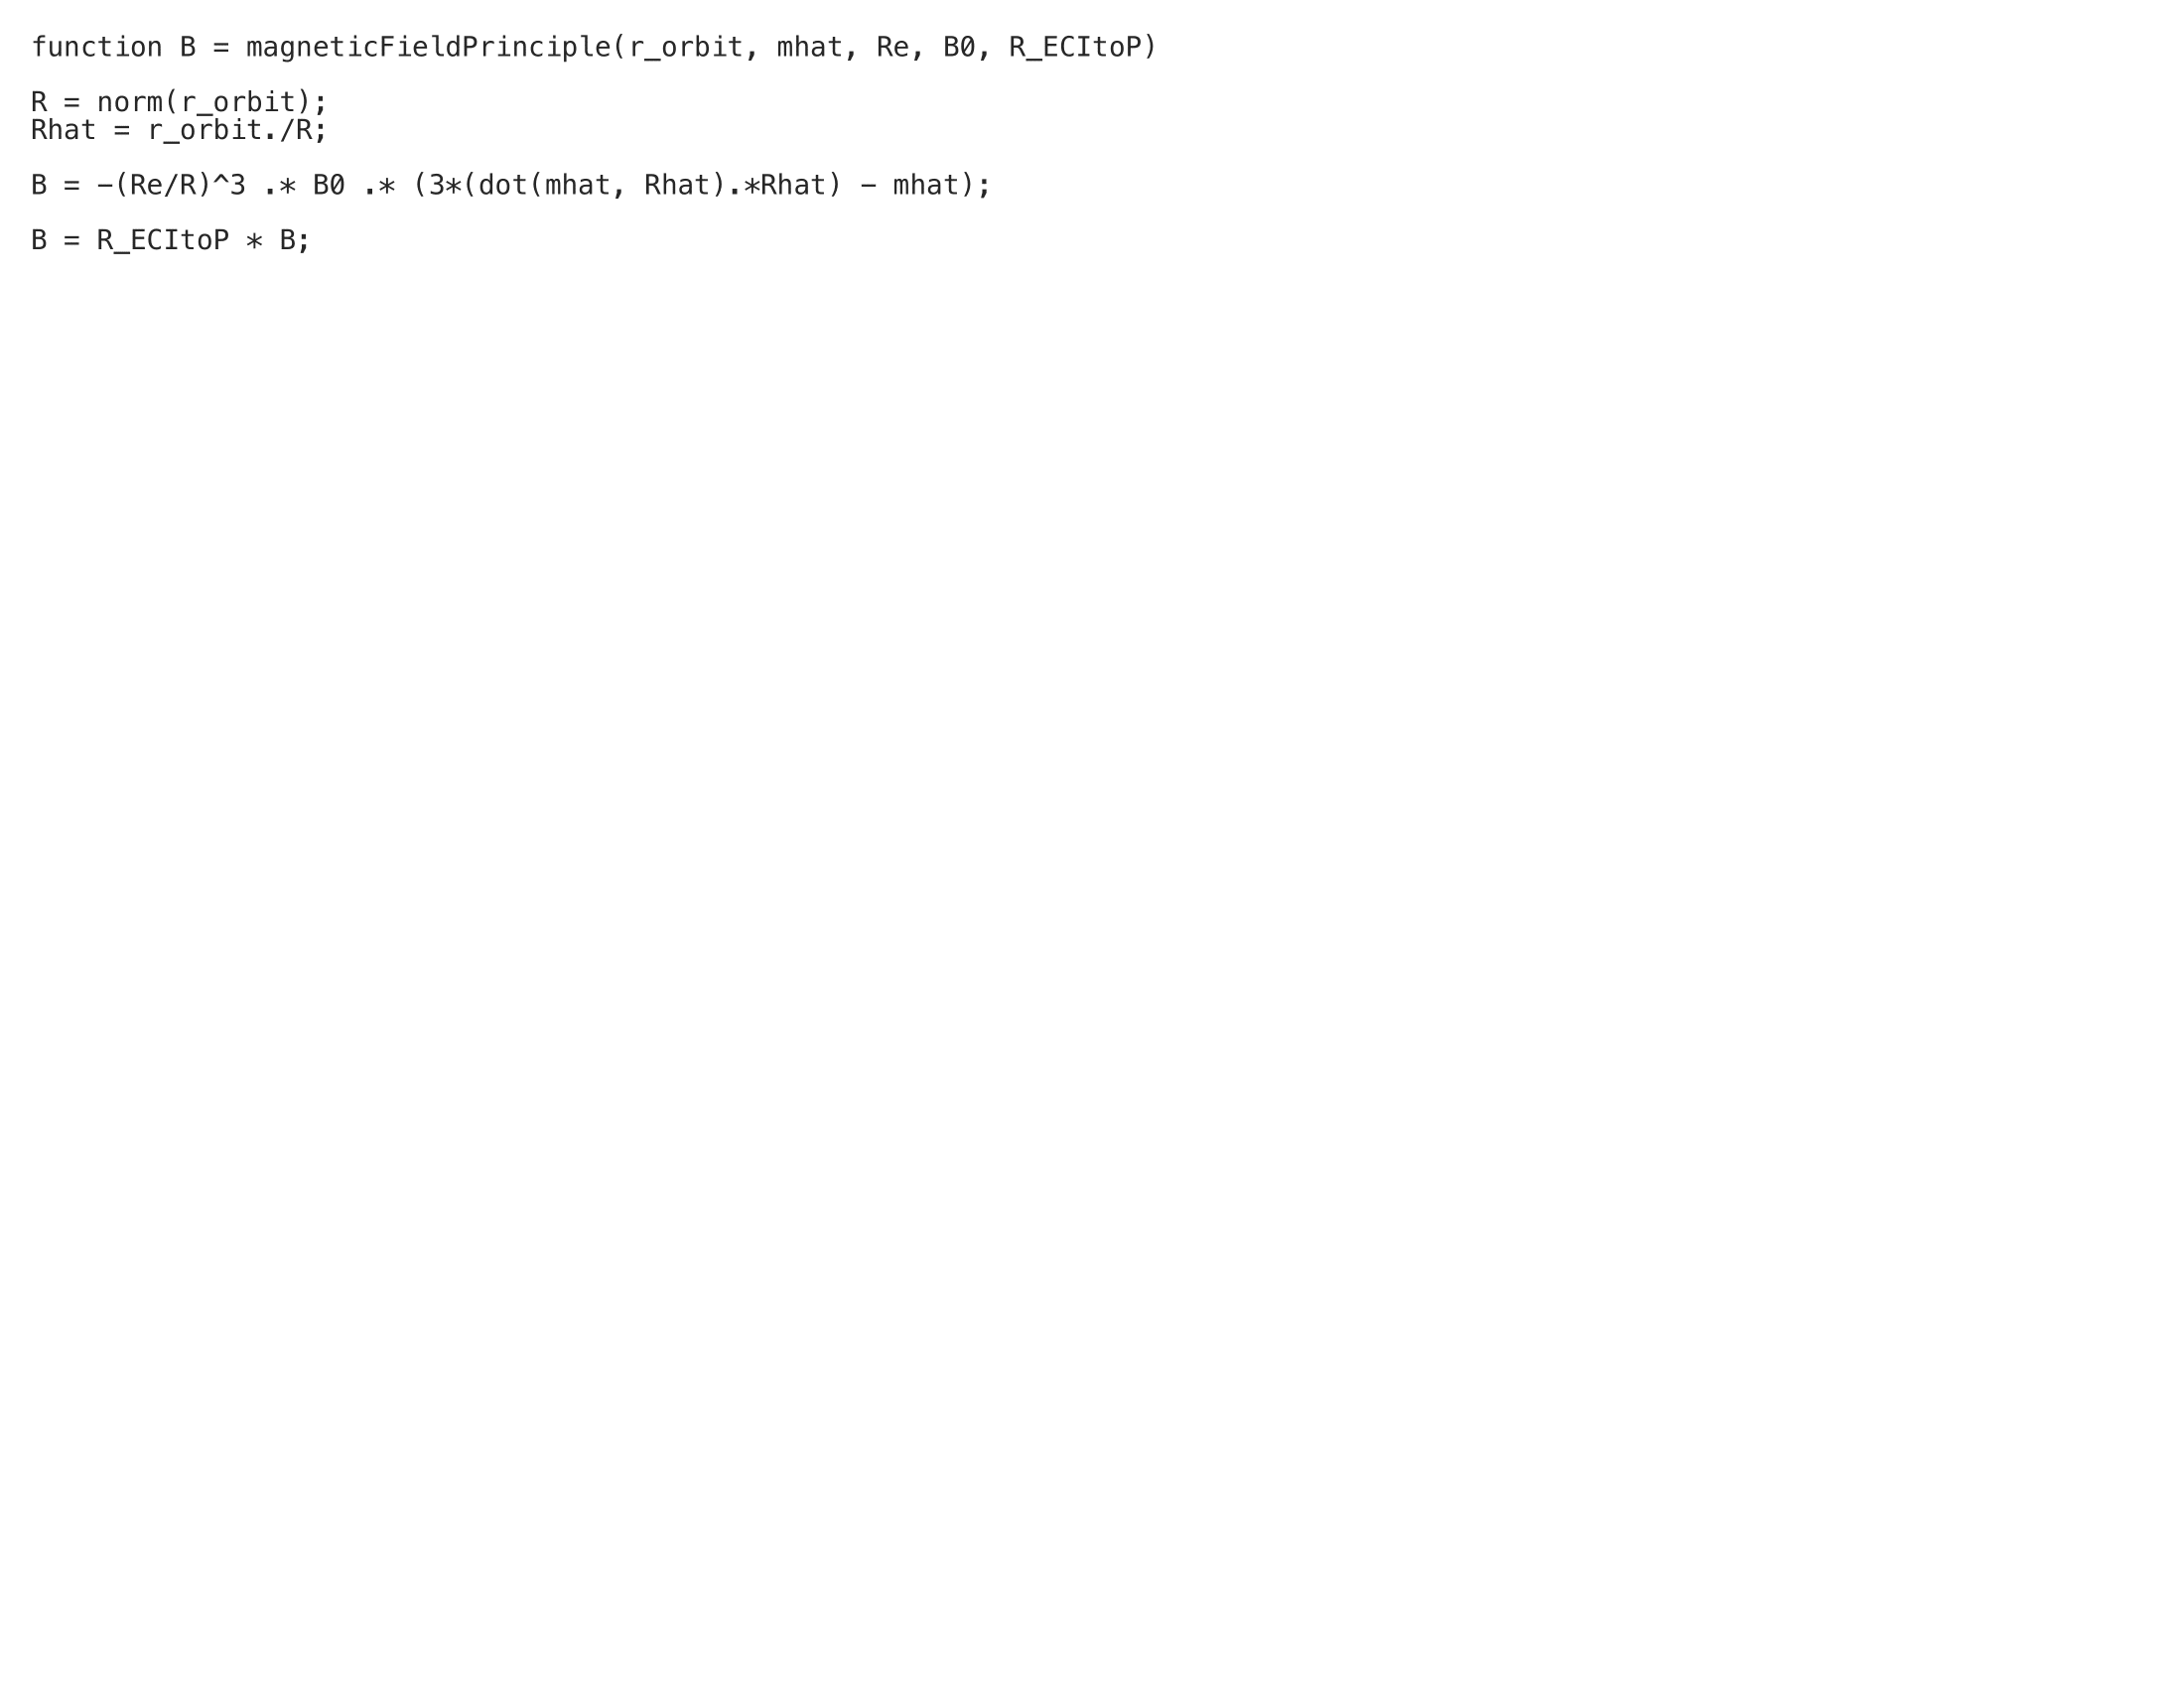
\includegraphics[trim={0cm 15cm 10cm 0cm},clip,width = 15cm]{Images/PS5/magneticField-5.png}
\end{figure}

\begin{figure}[H]
    \centering
    \captionsetup{justification = centering}
    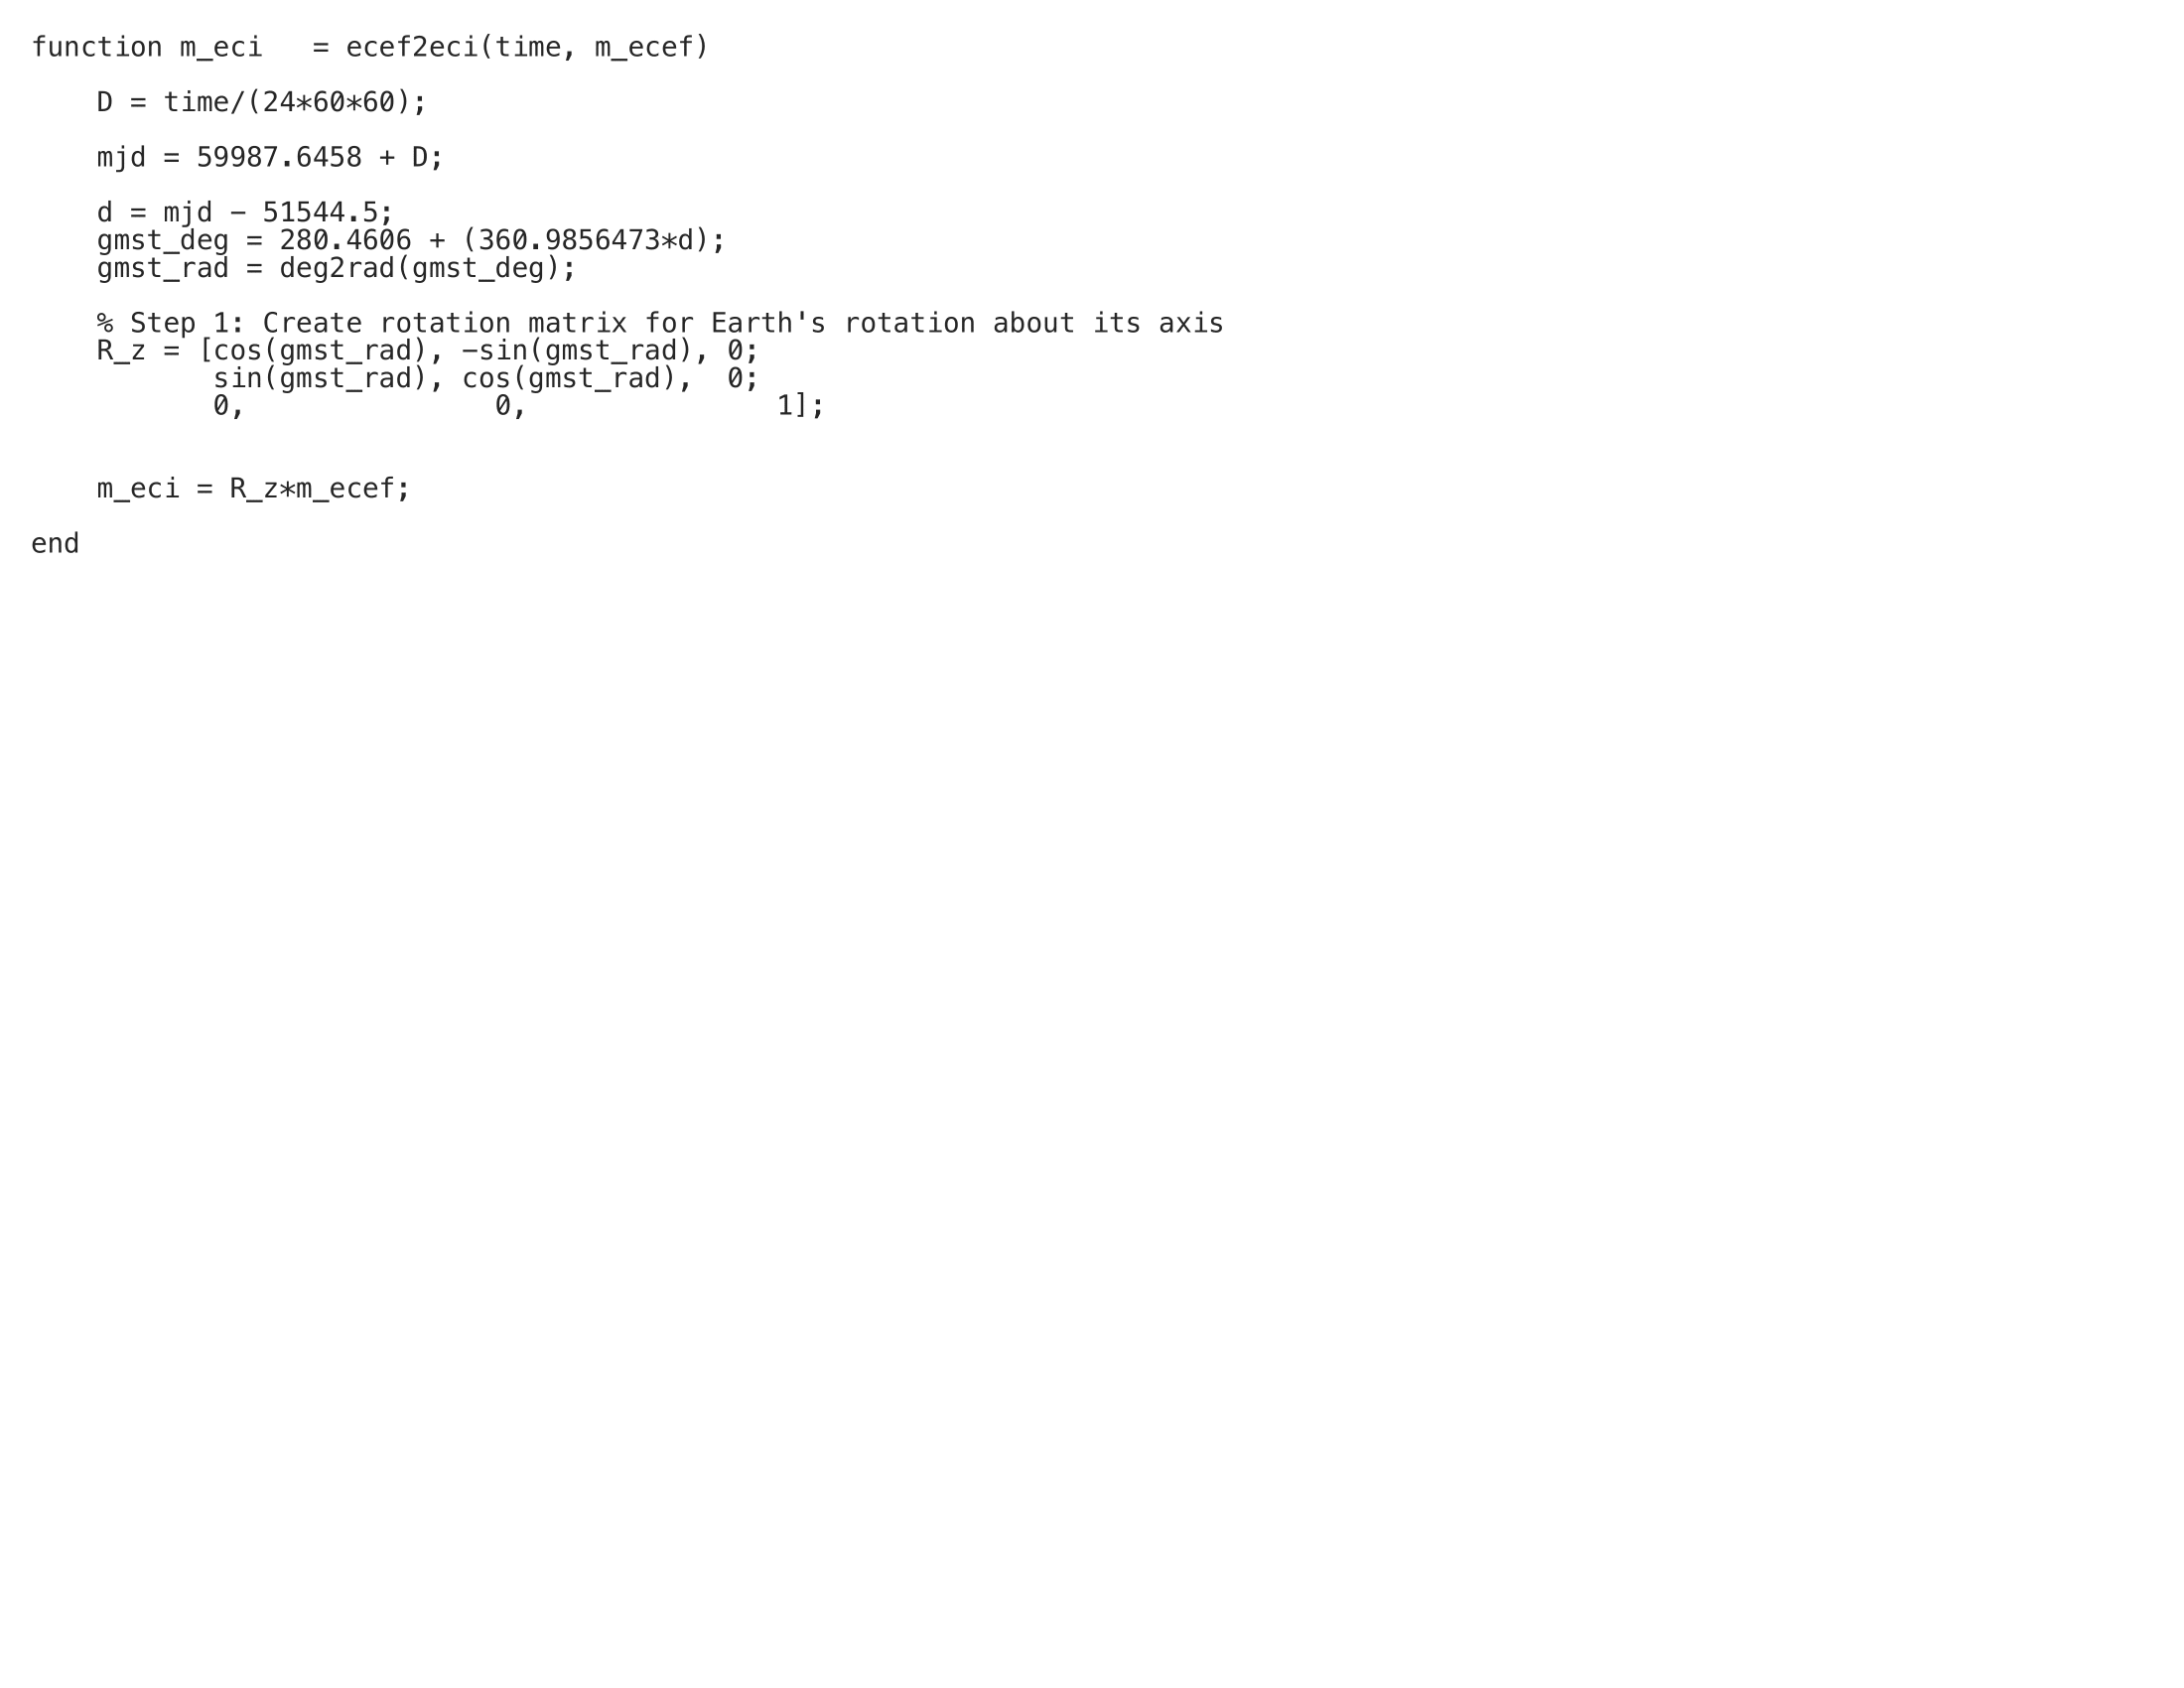
\includegraphics[trim={0cm 15cm 10cm 0cm},clip,width = 15cm]{Images/PS5/magneticField-6.png}
    \caption{Magnetic Dipole Model for Earth Magnetic Field Disturbance Torque}
    \label{fig:simulink_mag}
\end{figure}

\subsubsection{Solar Radiation Pressure}

To approximate the torque caused by solar radiation pressure, the surfaces of our satellite that were approximated in Homework 1 to have the properties shown in Figure \ref{fig:surface_labels} needed to be integrated over. Because each of our surfaces was approximated as being planar, the following equation was used to find the solar radiation force for each of the surfaces.

\begin{equation}
    - P A cos(\theta) * \left [ (1-c_s)\hat{\boldsymbol{S}} + 2 \left( c_s cos(\theta) + \frac{1}{3} c_d \right) \hat{\boldsymbol{N}} \right]
\end{equation}

In this equation, $P$ is the mean momentum flux, $A$ is the area of the surface, $c_s$ and $c_d$ are the spectral and diffusion coefficients respectively, $\hat{\boldsymbol{S}}$ is the unit vector in the direction of the sun, $\hat{\boldsymbol{N}}$ is the unit vector normal to the surface, and $\theta$ is the angle between $\hat{\boldsymbol{S}}$ and $\hat{\boldsymbol{N}}$. Because the satellite is in a sun synchronous orbit, $\hat{\boldsymbol{S}}$ was approximated as the cross product between the radius and velocity since the direction of the sun would be roughly normal to the orbital plane. Furthermore, since the orbit was specifically chosen to avoid eclipses, they didn't need to be accounted for in the model. To determine whether a given surface of the satellite was lit by the sun or not, the dot product was taken between $\hat{\boldsymbol{S}}$ and $\hat{\boldsymbol{N}}$. If it was positive (i.e. the vectors point in the same direction) then it was approximated that the entire surface was lit by the sun. Because of this, more accuracy in shadowing could be implemented in the future. More research needs to be done into the selections for $c_s$ and $c_d$ and as well as $P$. For the time being, $c_s$ and $c_d$ were approximated as $\frac{1}{3}$ by assuming that there were equal parts absorption, deflection, and spectral diffusion. Once the solar radiation force was calculated for each surface, the torque contribution was calculated by taking the cross product with the distance between the center of mass of the spacecraft and center of pressure of the surface. 

\begin{eqnarray} \label{eqn:torqueFromForce}
    \vec N = \sum^n_{i=1} \vec R_i \times \vec F_i
\end{eqnarray}

The following simulink models were implemented to calculate the moments for each of the surfaces.

\begin{figure} [H]
    \centering
    \begin{lstlisting}
function M = resultantSolarTorque(cd, cs, P, A, N, centroid, rcm, A_ptob, sunUnit)
M = zeros([3 1]);
n = size(A, 1);

%Rotate everything to principle frame
N = transpose(N);
centroid = transpose(centroid);
rcm = A_ptob.' * transpose(rcm);
for i=1:n
    N(:, i) = A_ptob.' * N(:, i);
    centroid(:, i) = A_ptob.' * centroid(:, i);
end 

for i=1:n
    if dot(N(:, i), sunUnit) > 0
        theta = asin(dot(sunUnit, N(:, i)));
        sun_force = -P*A(i)*cos(theta)*(1-cs);
        normal_force = -P*A(i)*cos(theta)*2*(cs*cos(theta) + (1/3*cd));
        total_force = sun_force + normal_force;
        M = M + cross(centroid(:, i) - rcm, total_force);
    end
end
end
    \end{lstlisting}
    \caption{Aerodynamic Torque}
    \label{fig:solar_drag_code}
\end{figure}

\begin{figure}[H]
    \centering
    \captionsetup{justification = centering}
    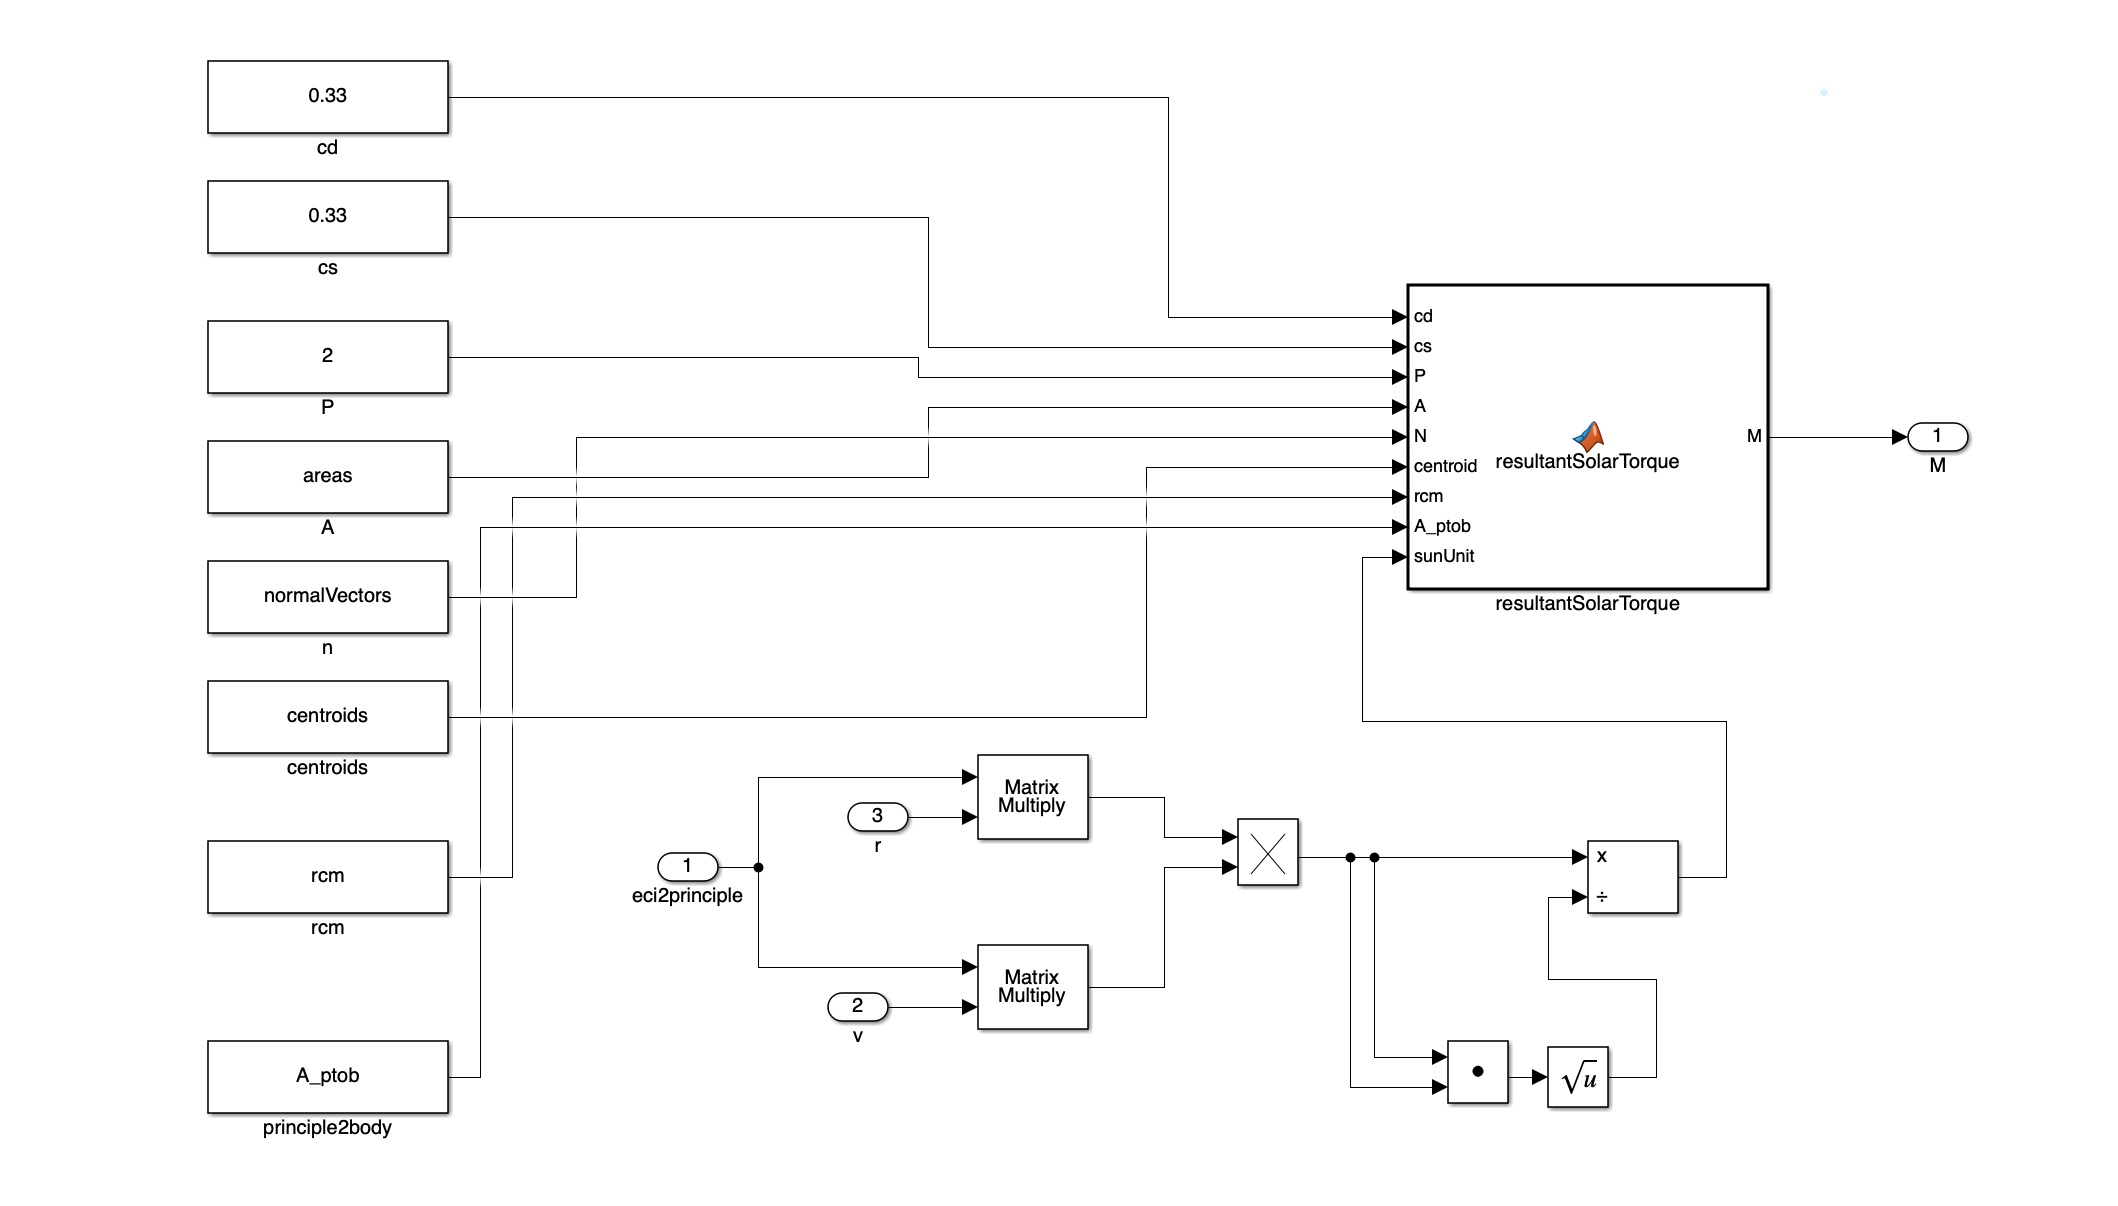
\includegraphics[width = 15cm]{Images/PS5/solarTorqueSimulink.png}
    \caption{Solar Radiation Pressure Model}
    \label{fig:simulink_sol}
\end{figure}

The above model only includes torques from the solar radiation pressure introduced directly from the sun. Contributions from Earth's reflectance and radiation were neglected.


\subsubsection{Atmospheric Drag}

Similarly to solar radiation, the atmospheric drag was modeled through first considering the aerodynamic force on each of the surfaces of our satellite that were approximated in Homework 1 and are summarized in Figure \ref{fig:surface_labels}. Because atmospheric drag only affects the portion of the satellite's surface that faces in the direction of the velocity vector, the dot product between each of the normal vector's for the surfaces and the velocity vector was taken. If it was positive, the surface was included in the force calculation. Because each of the surfaces of the satellite was approximated to be planar, the following equation was used for all of them.

\begin{equation}
    - \frac{1}{2} c_d \rho v^2 A ( \hat{\boldsymbol{N}} \cdot \hat{\boldsymbol{V}} ) \hat{\boldsymbol{V}}
\end{equation}

In this equation, $c_d$ was the coefficient of drag and was approximated as 2 and $\rho$ was found through interpolating the value for an altitude of 710 km from the text which was on the magnitude of $10^{-15}$. Similarly to solar radiation pressure, the torque was then found by taking the cross product between each of the resultant forces and the vector between the centers of gravity and pressure as in Equation \ref{eqn:torqueFromForce}.

The following simulink models were created to implement these functions.

\begin{figure}[H]
    \centering
    \captionsetup{justification = centering}
    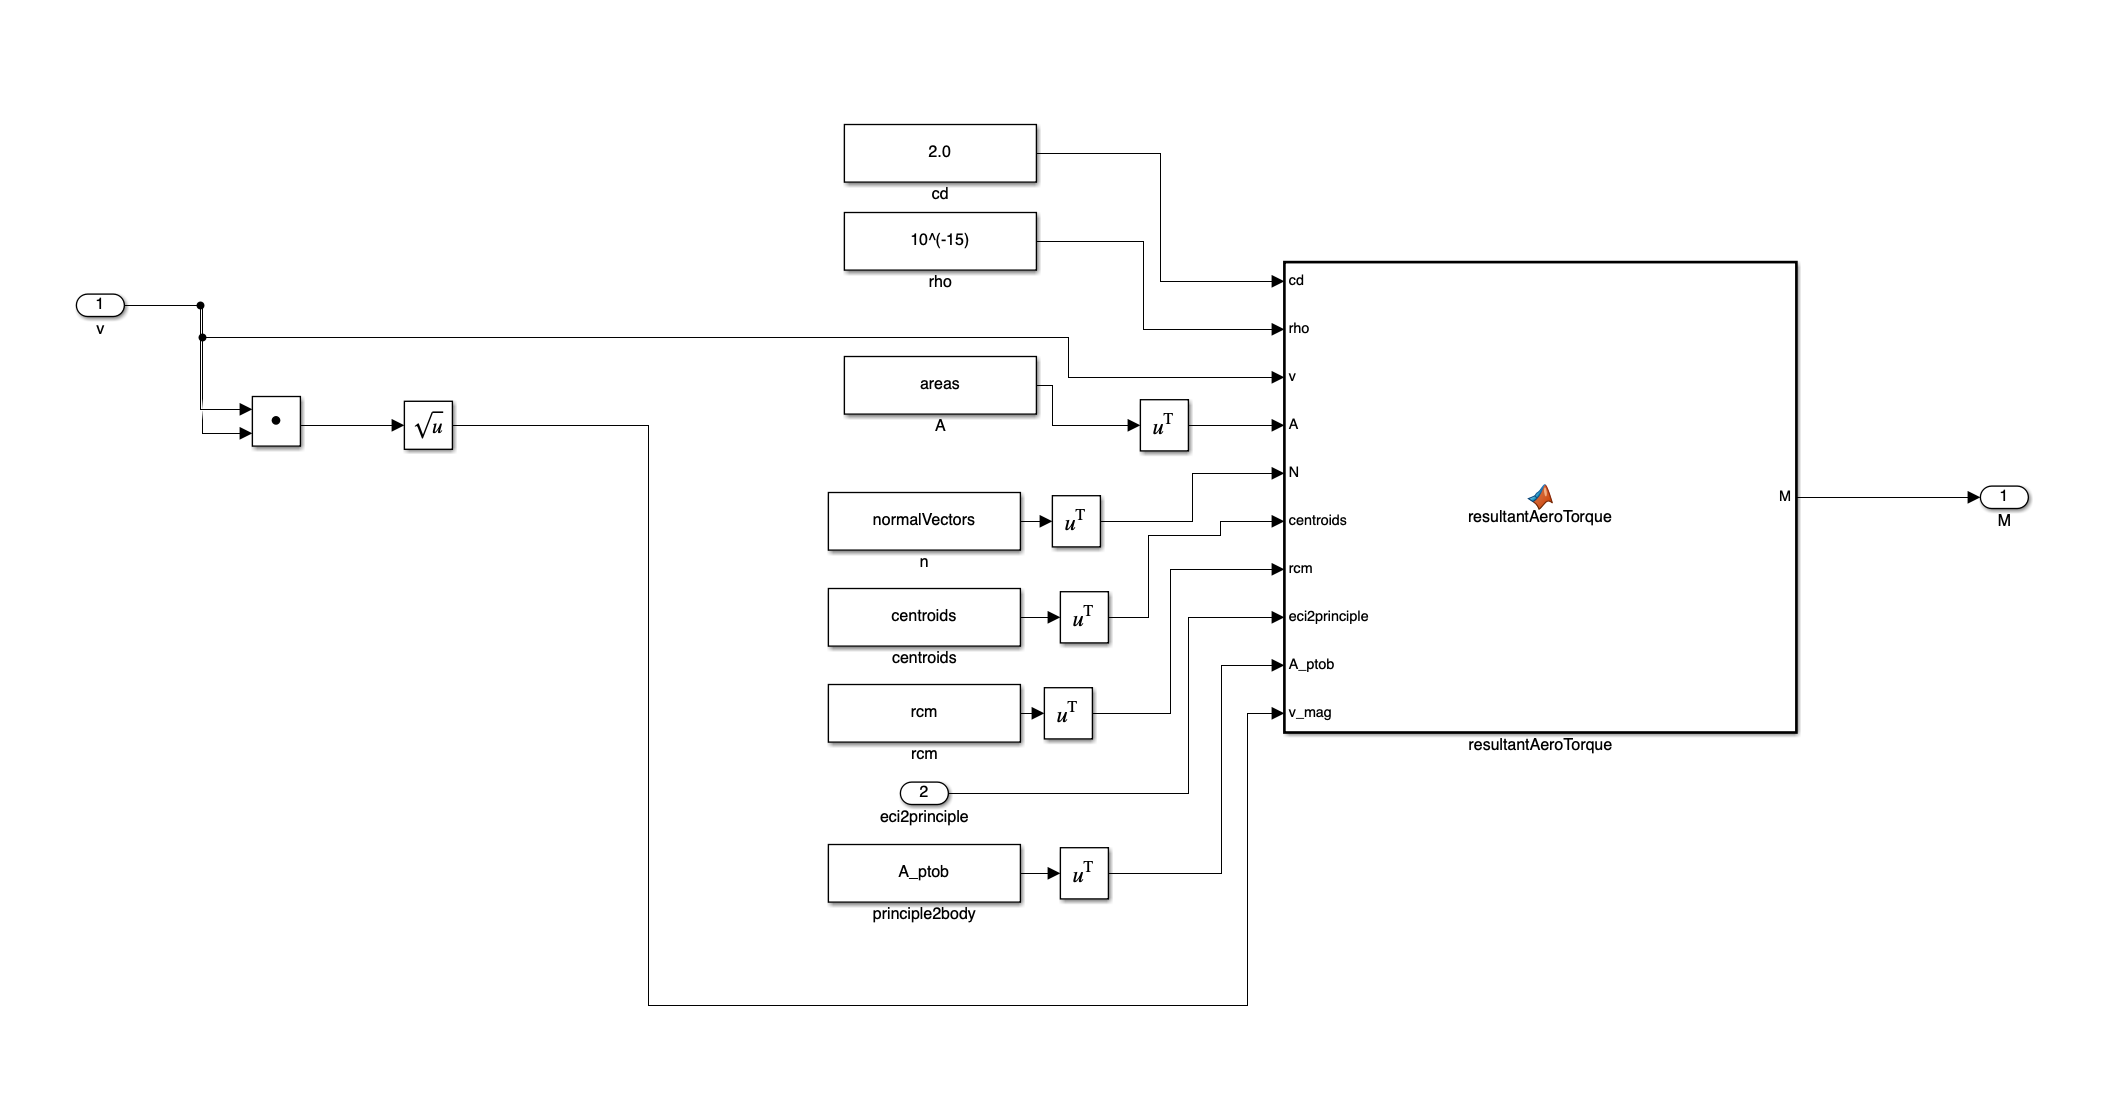
\includegraphics[width = 15cm]{Images/PS5/aeroTorqueSimulink.png}
    \caption{Atmospheric Drag Model}
    \label{fig:simulink_aero}
\end{figure}

\begin{figure} [H]
    \centering
    \begin{lstlisting}
function M = resultantAeroTorque(cd, rho, v, A, N, centroids, rcm, eci2principle, A_ptob, v_mag)
force = zeros([3 1]);
M = zeros([3 1]);
n = size(A, 1);

%Rotate everything to principle frame
v = eci2principle*v;
rcm = A_ptob * rcm;
for i=1:n
    N(:, i) = A_ptob * N(:, i);
    centroids(:, i) = A_ptob * centroids(:, i);
end 


vUnit = v ./ v_mag;
disp(dot(N(1, :), vUnit))

for i=1:n
    if dot(N(:, i), vUnit) > 0
        force = -0.5 .* cd .* rho .* v_mag^2 .* A(i) .* dot(N(:, i), vUnit) .* vUnit;
        M = M + cross(centroids(:, i) - rcm, force);
    end
end
    \end{lstlisting}
    \caption{Aerodynamic Torque}
    \label{fig:aero_drag_simulink_code}
\end{figure}



\subsection{Include all torques you have been able to model in numerical integration. Please show comparison of numerically computed disturbance torques with expected values and trend from theory (model) and tables (Wertz) referenced in class. Plot all torque components in principal axes over time. Plot the resultant (sum) of all torques in principal axes.}

The only torque that was fully modeled was the magnetic torque. In the following figure, the oscillating lines show the numerically integrated torque and the lower and upper bounds are from the following equation shown in class.

\begin{equation}
    m B_{max} = 2 m \frac{R_e^2 B_0}{R^3}
\end{equation}

\begin{figure}[H]
    \centering
    \captionsetup{justification = centering}
    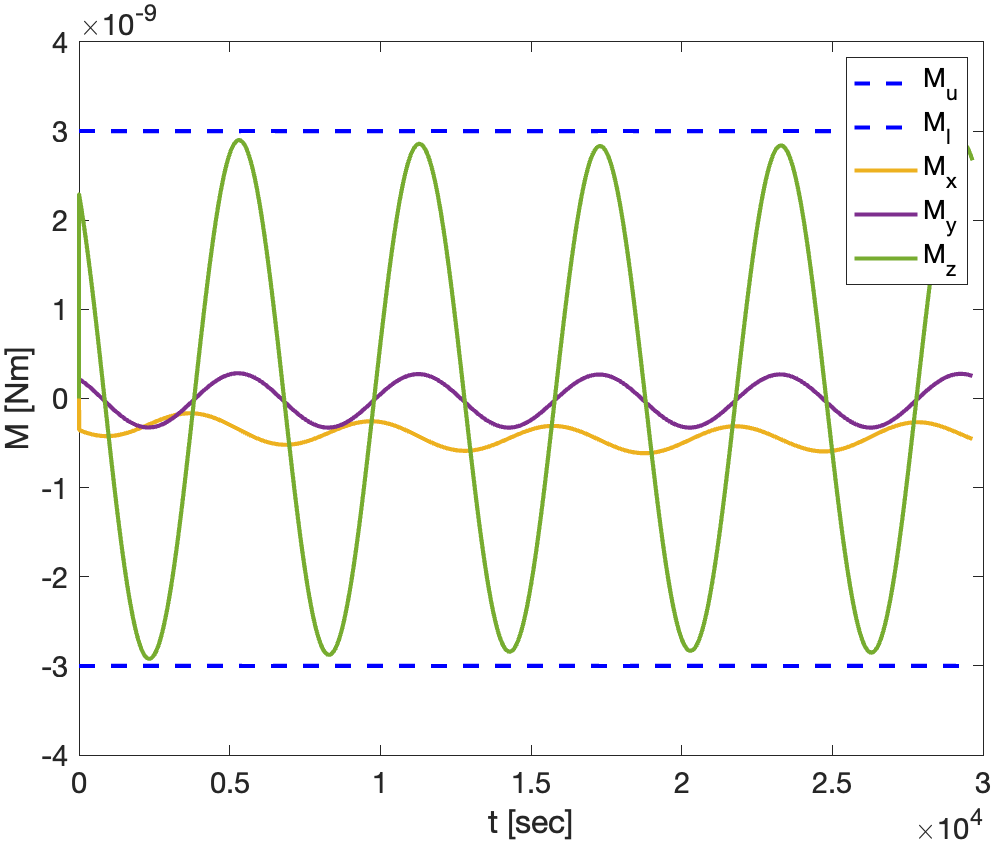
\includegraphics[width = 15cm]{Images/PS5/magnetic_torque.png}
    \caption{Torque from Magnetic Disturbances}
    \label{fig:simulink_sol}
\end{figure}

The torques stay within the lower and upper bounds and follow an oscillatory pattern as expected.